\chapter[Empirical Data Analysis]{Empirical Data Analysis}
\label{cp:application}

This chapter applies the proposed FARFIMA order-selection and forecasting framework to two French demographic applications. The first considers age-specific fertility-rate increments, while the second considers female and male log-mortality rates. Both datasets have a natural functional structure because each annual observation is a curve indexed by age.

The empirical analysis smooths the noisy age-specific rates before modelling them as functional observations \citep{HU07,RH09}. The fertility curves are smoothed across age using weighted regression B-splines with a concavity constraint and smoothing parameter $\lambda=0.4$; the annual fertility-rate increments are then calculated from the smoothed curves. For mortality, invalid rates are first interpolated over time within each age and transformed to the base-10 logarithmic scale. Female and male log-mortality curves are subsequently smoothed across age using weighted penalised regression splines with a monotonicity constraint above age 65. Rainbow plots display the temporal evolution of the raw and smoothed curves as in \citet{YS25}. For each application, the functional autocorrelation function (fACF) of \citet{GJ21} and the stationarity test of \citet{LPG14} assess persistence, while the bias-corrected LPWN estimator determines the fractional order. After data preprocessing, three forecasting methods are evaluated: the FARFIMA$(1,1,0)$ benchmark, the proposed functional information criterion (Functional IC), and expanding-window cross-validation (CV). Their performance is assessed using expanding-window forecasts and the point and interval criteria introduced in Chapter~\ref{cp:method}.

\section{Forecasting Design}
\label{sec:emp-forecast-design}

The forecasting experiment compares three methods. The benchmark is a FARFIMA$(1,1,0)$ model with $d=1$. For the other two methods, the fractional order $d$ is first estimated using the bias-corrected LPWN estimator. Conditional on this estimate, Functional IC selects the short-memory orders $(p,q)$ using the proposed adaptive functional information criterion, whereas CV selects $(p,q)$ by expanding-window cross-validation. The estimated fractional order and the selected short-memory orders are fixed before evaluation on the test sample.

For each series, the first 70\% of curves form the training sample, the next 15\% form the validation sample, and the final 15\% form the test sample. The models are fitted to the smoothed curves, and forecasts are produced using an expanding estimation window for horizons $h=1,\ldots,10$. All point and interval forecasting metrics are evaluated against the corresponding raw observations, so the evaluation incorporates both errors in forecasting the underlying smooth curves and observation-level variation. Candidate orders satisfy $0\leq p,q\leq5$, excluding $(0,0)$, while the memory estimator uses one principal component, the empirical covariance operator, 399 bootstrap replications, and a fractional-differencing trim of 20. To quantify forecast uncertainty, split conformal prediction intervals with nominal coverage probabilities of 80\% and 95\% are constructed from the smoothed curves and calibrated using the validation sample.

\section{Empirical Studies}
\label{sec:emp-studies}

\subsection{French Fertility-Rate Changes}
\label{sec:emp-fertility}

\subsubsection{Data source and preprocessing}

The fertility data are annual age-specific fertility rates for France obtained from the Human Fertility Database \citep{HFD26}. The dataset and its country documentation are available from the \href{https://www.humanfertility.org/Country/Country?cntr=FRATNP}{Human Fertility Database France page}. The archived sample used in this study covers 1946--2022 and contains one curve for each year over ages 15--49.

Let $F_t(u)$ denote the fertility rate at age $u$ in year $t$. The analysis focuses on the symmetric relative change
\begin{equation}
    C_t(u)
    =
    \frac{2\{F_{t-1}(u)-F_t(u)\}}
         {F_{t-1}(u)+F_t(u)},
    \qquad t=1947,\ldots,2022.
    \label{eq:emp-fertility-change}
\end{equation}
Thus, $C_t(u)>0$ indicates a decline in the age-specific fertility rate from year $t-1$ to year $t$, whereas $C_t(u)<0$ indicates an increase. The transformation reduces the influence of the overall scale and produces 76 annual change curves.

The archived smoothed fertility curves are used for model estimation. The smoothing follows the functional demographic approach of estimating a smooth age profile in each year, with population-based weights accounting for heterogeneous measurement variability \citep{HU07}. Equation~\eqref{eq:emp-fertility-change} is calculated separately from the raw and smoothed rates. Models are fitted to the smoothed changes, while forecast accuracy is evaluated against the raw changes.

Figure~\ref{fig:emp-fertility-rainbow} compares the raw and smoothed fertility rates and their corresponding changes. Both versions show a clear shift of the modal childbearing age towards older ages and a reduction in the peak fertility rate. Smoothing removes local age-specific variation while retaining this evolution. The change curves fluctuate around zero across most ages but are more variable near the boundaries, where the fertility rates in the denominator of \eqref{eq:emp-fertility-change} are small.

\begin{figure}[!htb]
\centering
\begin{subfigure}[t]{0.48\textwidth}
\centering
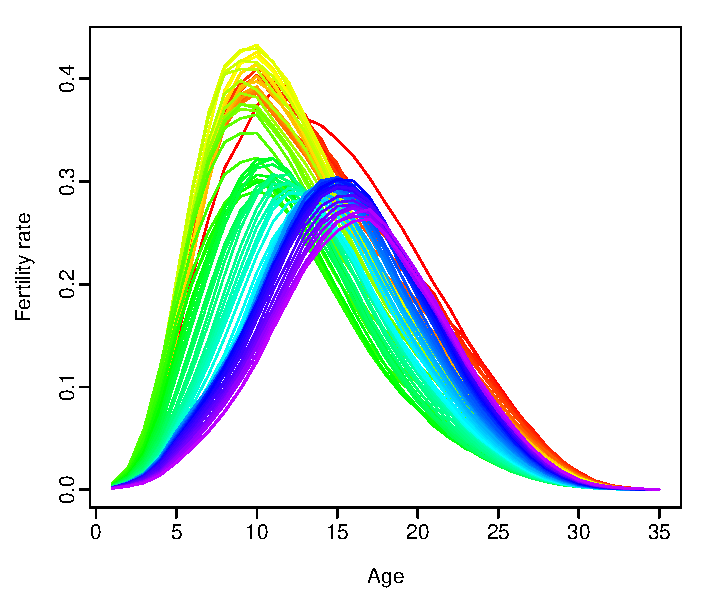
\includegraphics[width=\textwidth]{Figures/Empirical/France_fertility_raw_rainbow_plot.pdf}
\caption{Raw fertility rates}
\end{subfigure}
\hfill
\begin{subfigure}[t]{0.48\textwidth}
\centering
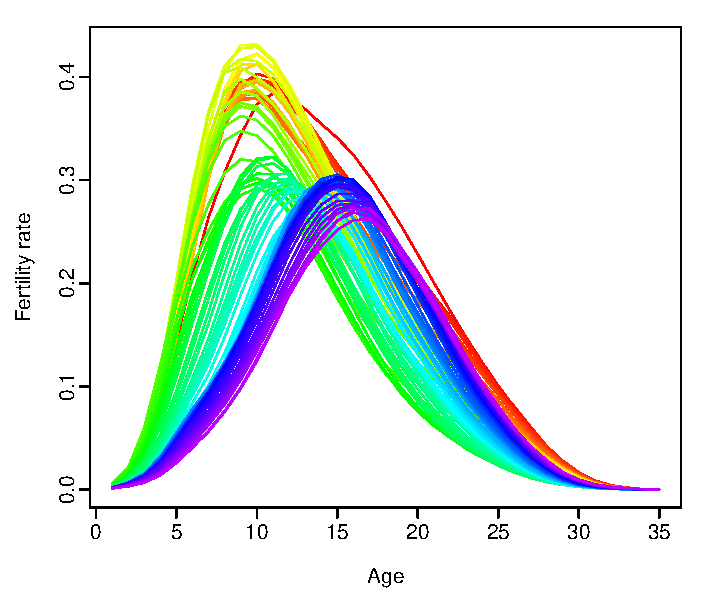
\includegraphics[width=\textwidth]{Figures/Empirical/France_fertility_smooth_rainbow_plot.pdf}
\caption{Smoothed fertility rates}
\end{subfigure}

\vspace{0.25cm}

\begin{subfigure}[t]{0.48\textwidth}
\centering
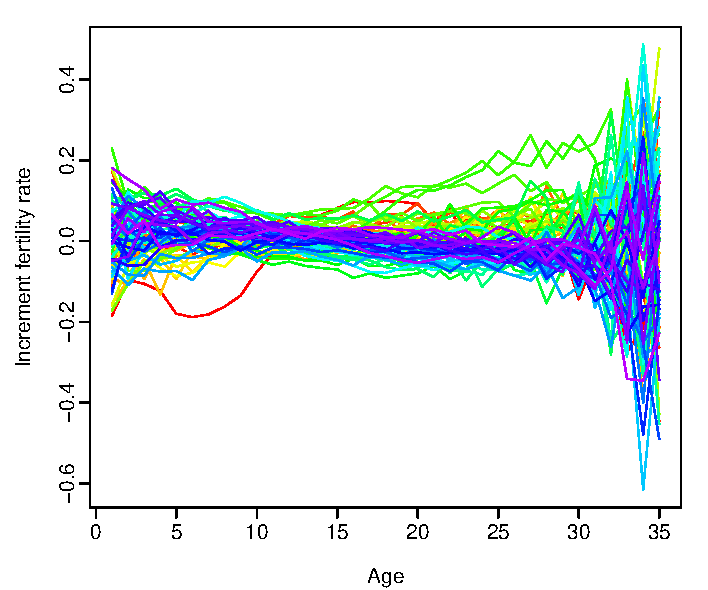
\includegraphics[width=\textwidth]{Figures/Empirical/France_fertility_raw_change_rainbow_plot.pdf}
\caption{Raw increment fertility rate}
\end{subfigure}
\hfill
\begin{subfigure}[t]{0.48\textwidth}
\centering
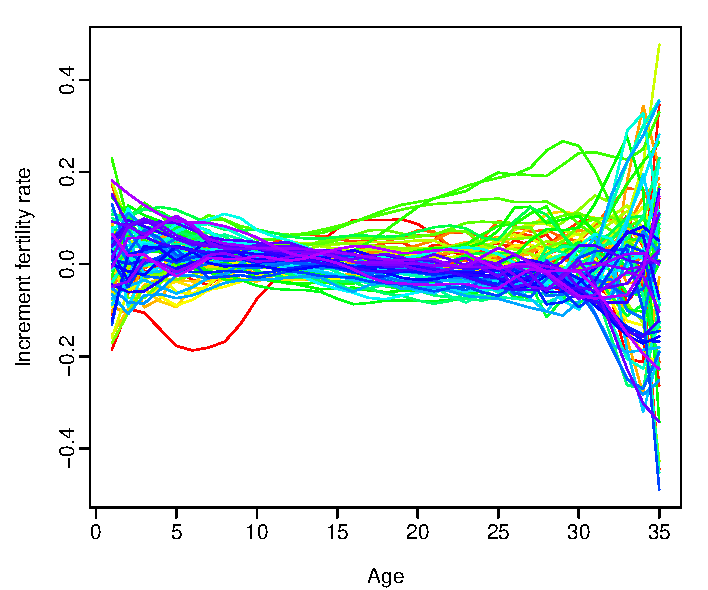
\includegraphics[width=\textwidth]{Figures/Empirical/France_fertility_smooth_change_rainbow_plot.pdf}
\caption{Smoothed increment fertility rate}
\end{subfigure}
\caption{\small Rainbow plots of the raw and smoothed French age-specific fertility rates and their increments. Curves run chronologically from the earliest years in red to the most recent years in violet.}
\label{fig:emp-fertility-rainbow}
\end{figure}

Figure~\ref{fig:emp-fertility-facf} shows that the fACF decays gradually across the lags rather than displaying an abrupt short-memory cut-off, which is consistent with long-range dependence. The stationarity test takes stationarity as its null hypothesis. With a $p$-value of 0.177, the null is not rejected, so the fertility-rate increments are treated as a stationary long-memory functional time series.

\begin{figure}[!htb]
\centering
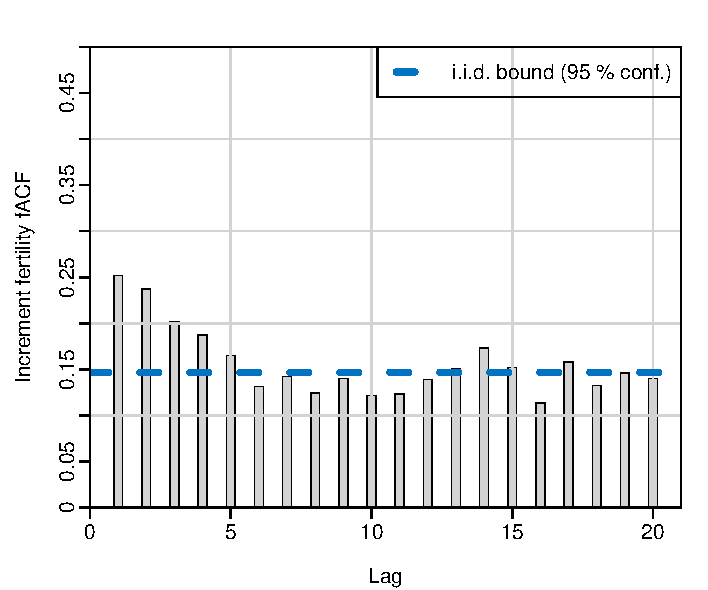
\includegraphics[width=0.62\textwidth]{Figures/Empirical/France_fertility_change_facf.pdf}
\caption{\small Functional autocorrelation function of the French fertility-rate changes. The dashed blue line is the simulated upper 95\% white-noise bound.}
\label{fig:emp-fertility-facf}
\end{figure}

\subsubsection{Forecasting results}

The BC-LPWN estimate is $\widehat d=0.3886$, which lies in the stationary long-memory range $0<d<1/2$. Conditional on this estimate, Functional IC selects $(p,q)=(1,0)$ and CV selects $(1,1)$. Thus, the two methods use the same fractional estimate and similar short-memory orders.

Figure~\ref{fig:emp-fertility-point-ratios} shows that the RMSE and MAE ratios of Functional IC and CV are below one at every horizon. The two methods give almost identical results. The ratios fluctuate over the first five horizons and generally decline from $h=6$ onward, indicating larger improvements at longer horizons. At $h=10$, the RMSE and MAE reductions are approximately 36\% and 32\%, respectively. The two selected orders therefore give nearly the same point forecast accuracy.

\begin{figure}[!htb]
\centering
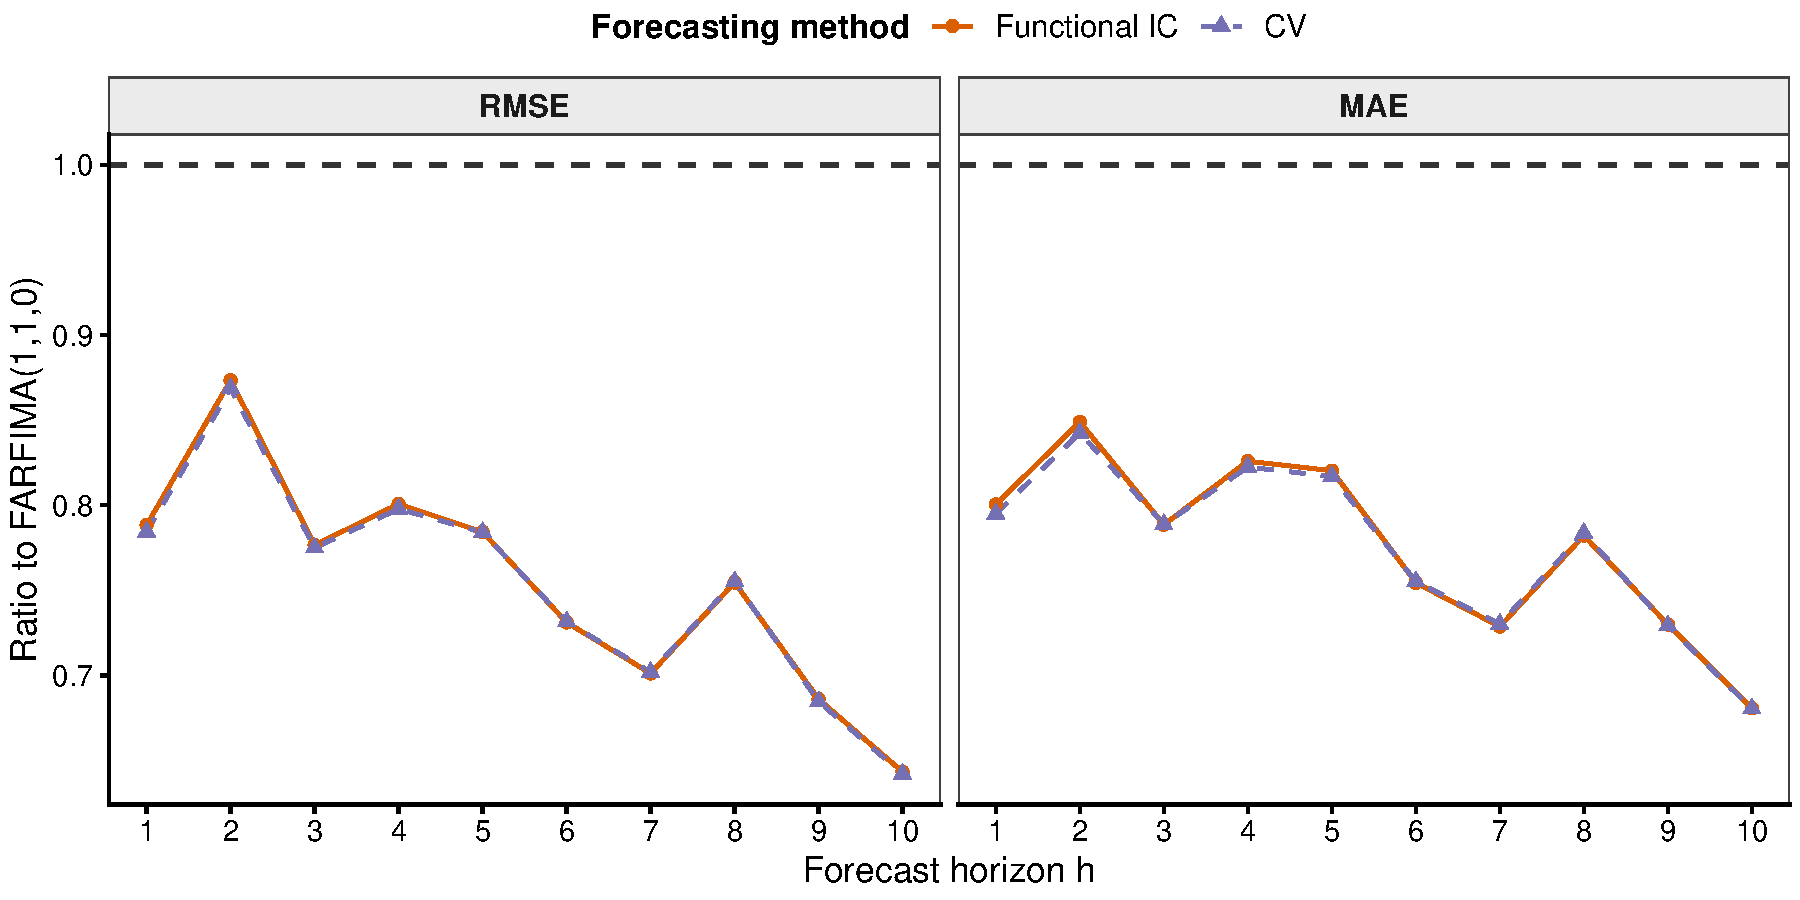
\includegraphics[width=0.98\textwidth]{Figures/Empirical/France_fertility_point_forecast_ratios.pdf}
\caption{\small RMSE and MAE ratios to FARFIMA$(1,1,0)$ for French fertility-rate increments. Values below one indicate improvement over FARFIMA$(1,1,0)$.}
\label{fig:emp-fertility-point-ratios}
\end{figure}

Figure~\ref{fig:emp-fertility-ecp} presents the corresponding coverage results. The 95\% intervals from Functional IC and CV attain coverage close to or above the nominal level at most horizons. Their 80\% intervals also tend to exceed the nominal level, particularly at the middle horizons.

\begin{figure}[!htb]
\centering
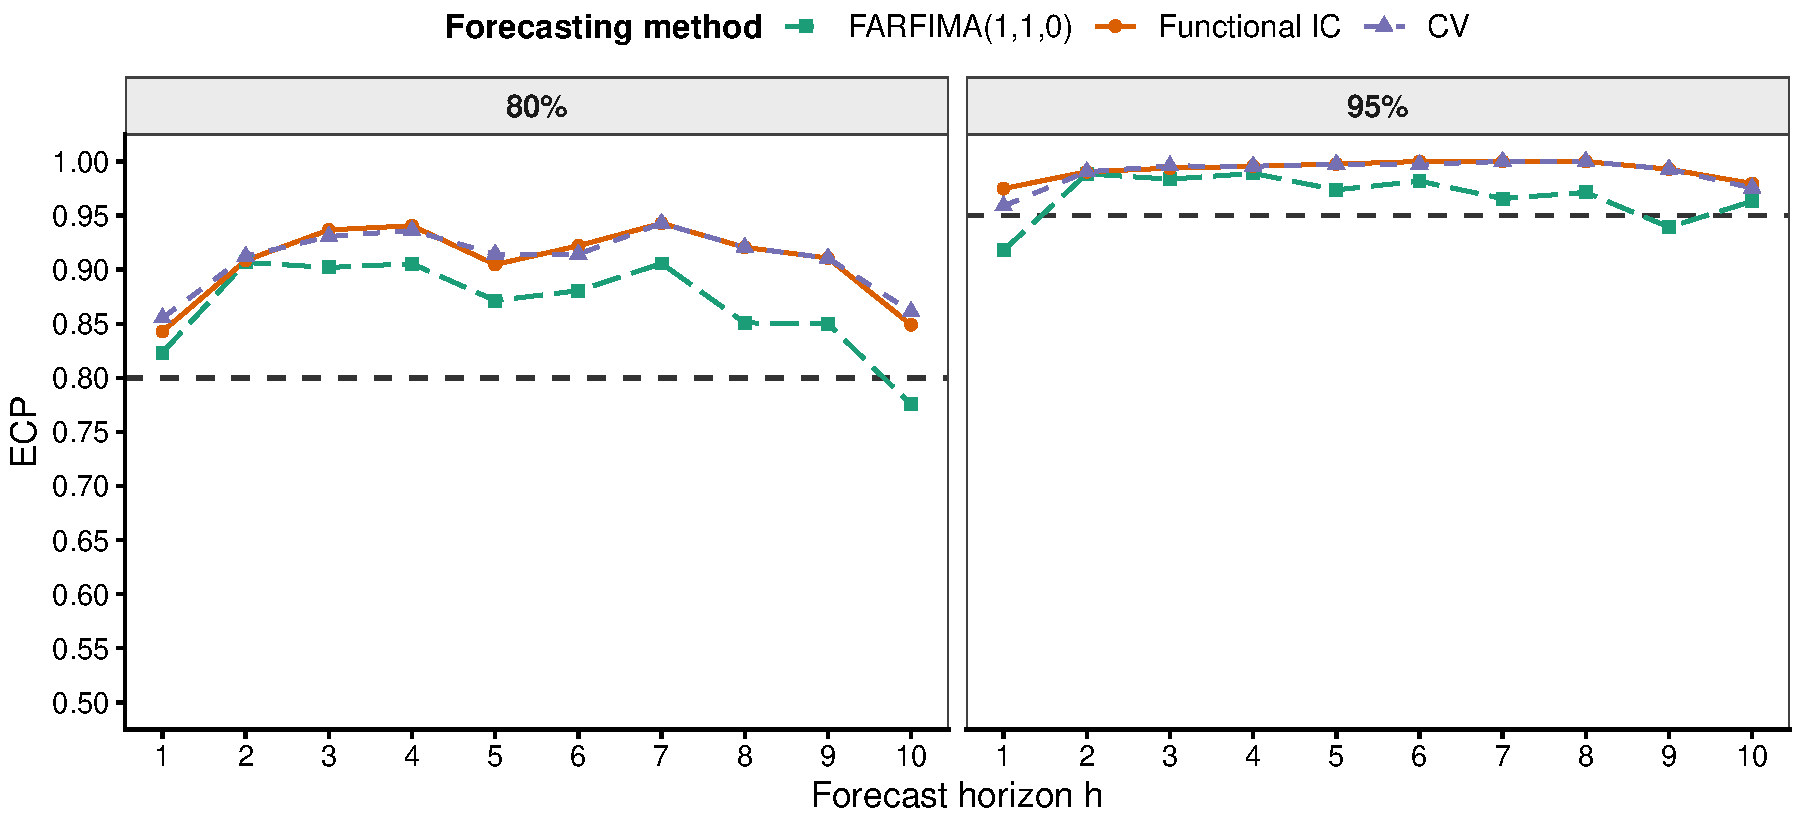
\includegraphics[width=0.98\textwidth]{Figures/Empirical/France_fertility_ecp.pdf}
\caption{\small Empirical coverage probabilities for the 80\% and 95\% prediction intervals for French fertility-rate increments. Horizontal lines indicate the nominal coverage probabilities.}
\label{fig:emp-fertility-ecp}
\end{figure}

Figures~\ref{fig:emp-fertility-is-ratios} and \ref{fig:emp-fertility-wis-ratios} show the interval score and weighted interval score ratios. For both coverage levels, the interval score ratios are below one at almost every horizon. The 95\% ratio is close to one at $h=8$ and is substantially lower at $h=9$ and $h=10$. The weighted interval score ratios remain below one throughout and reach approximately 0.69 at $h=10$. Functional IC and CV again give very similar results. These score ratios should be considered together with the over-coverage shown in Figure~\ref{fig:emp-fertility-ecp}.

\begin{figure}[!htb]
\centering
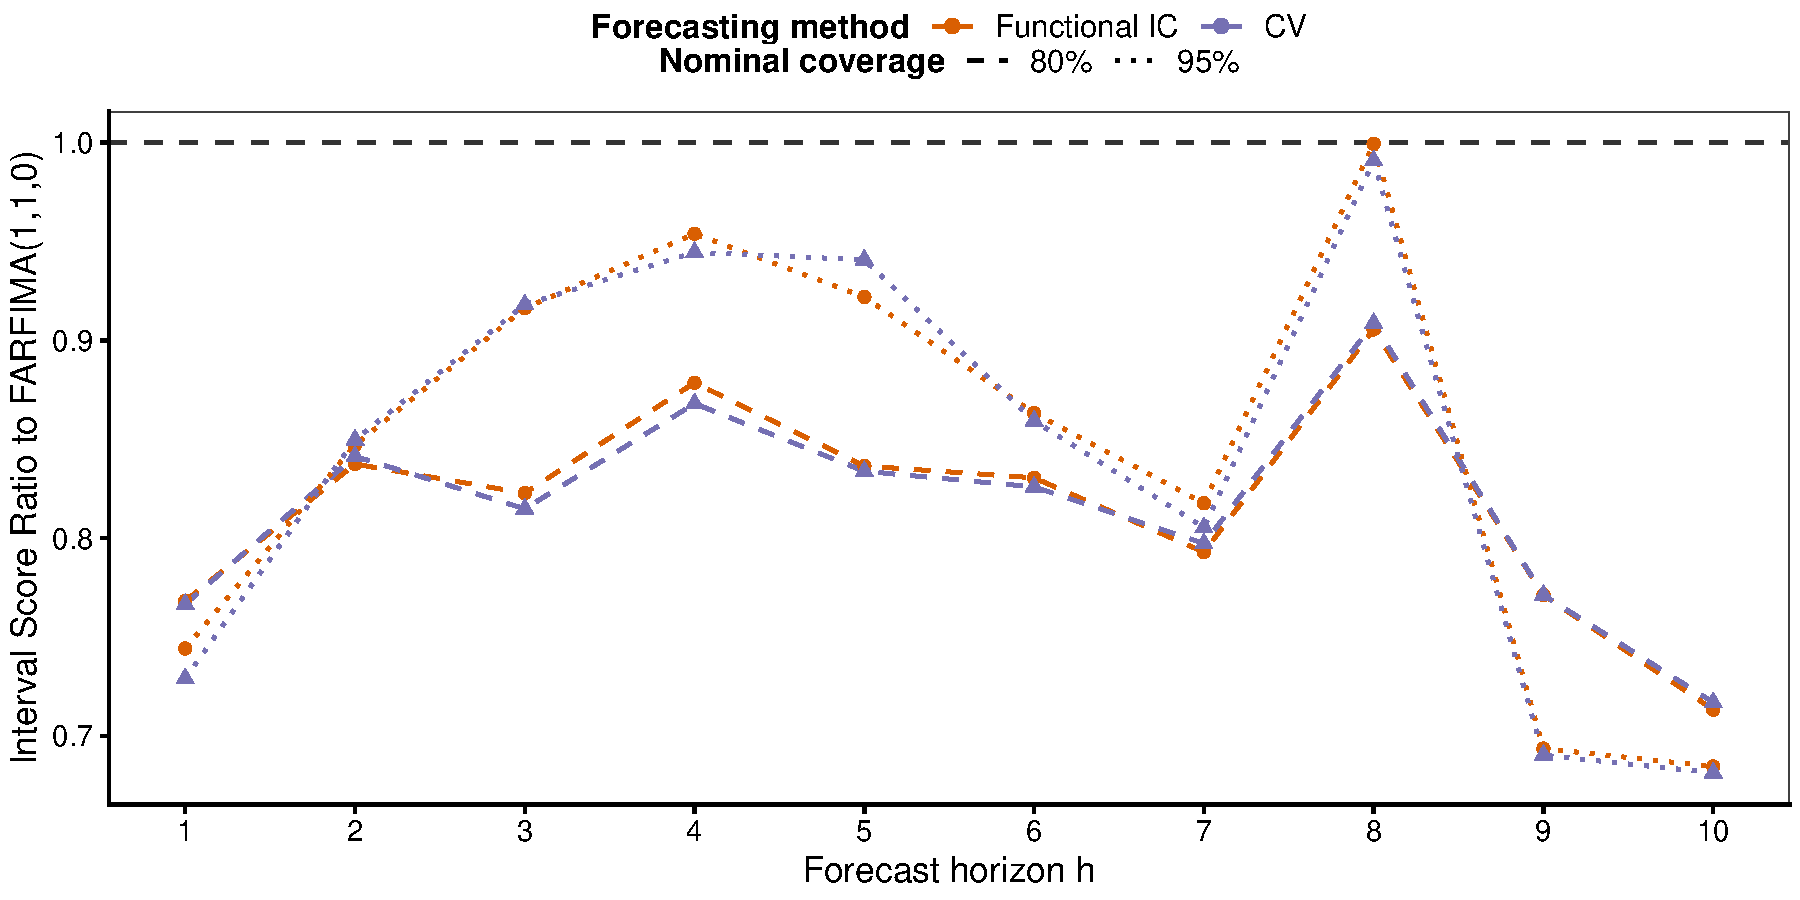
\includegraphics[width=0.98\textwidth]{Figures/Empirical/France_fertility_interval_score_ratios.pdf}
\caption{\small Interval Score Ratio to FARFIMA$(1,1,0)$ for French fertility-rate increments. The 80\% and 95\% prediction intervals are distinguished by line type. Values below one indicate improvement over FARFIMA$(1,1,0)$.}
\label{fig:emp-fertility-is-ratios}
\end{figure}

\begin{figure}[!htb]
\centering
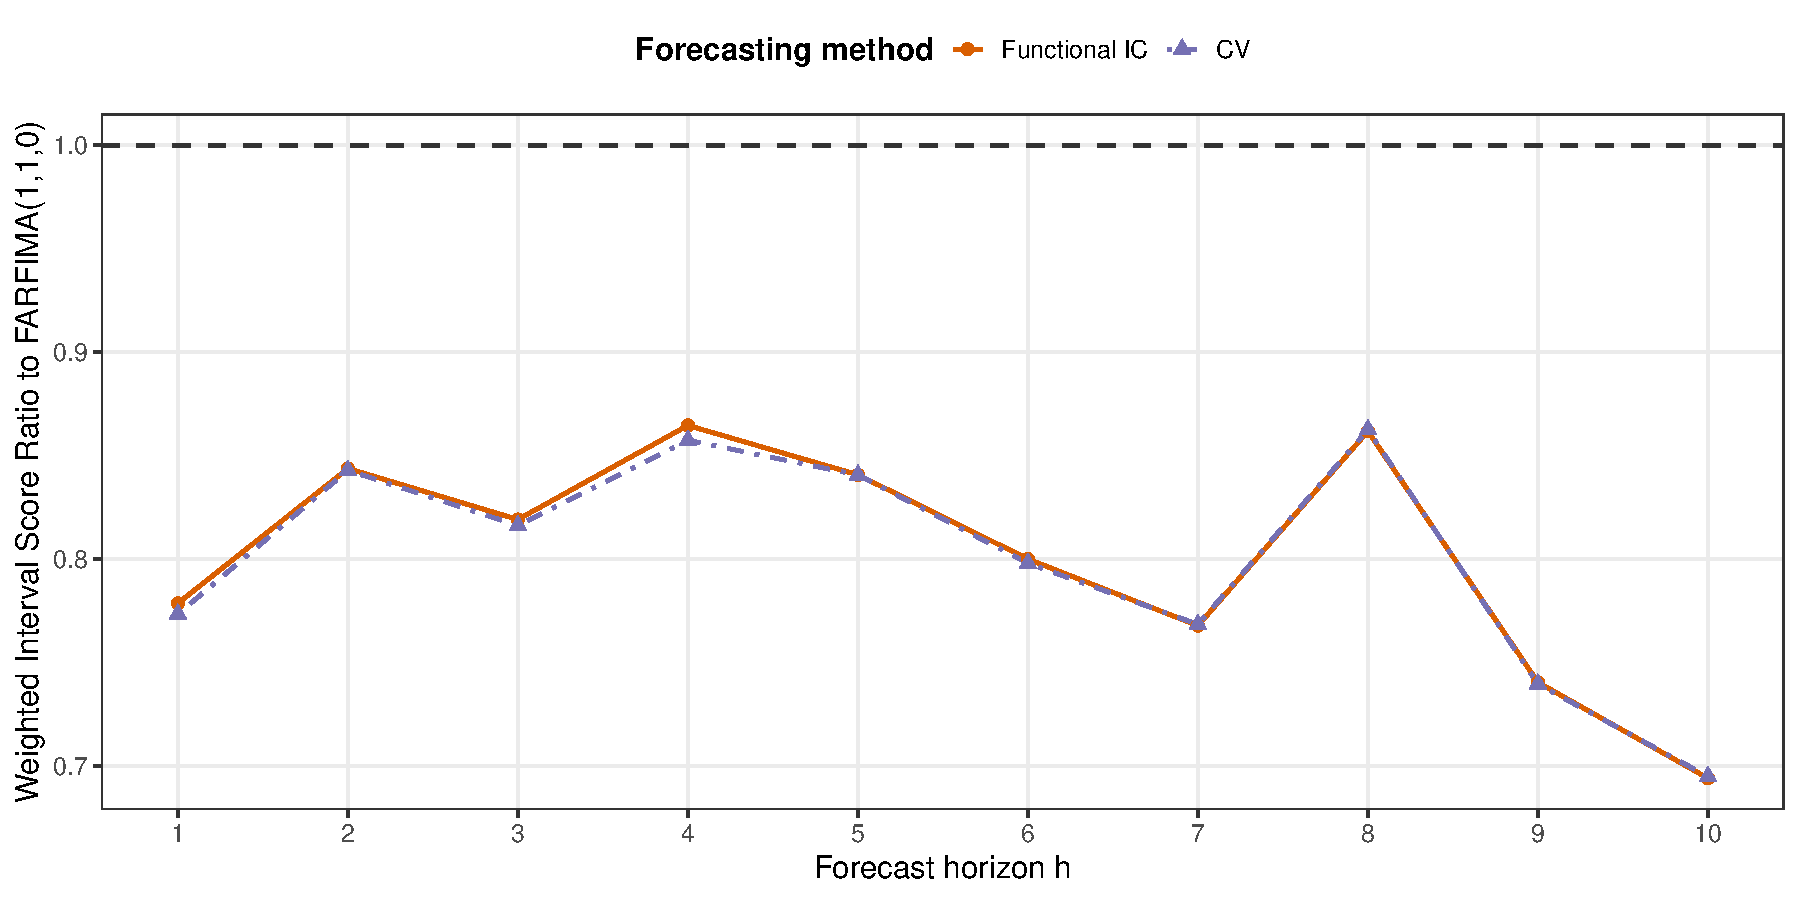
\includegraphics[width=0.98\textwidth]{Figures/Empirical/France_fertility_weighted_interval_score_ratios.pdf}
\caption{\small Weighted Interval Score Ratio to FARFIMA$(1,1,0)$ for French fertility-rate increments. Values below one indicate improvement over FARFIMA$(1,1,0)$.}
\label{fig:emp-fertility-wis-ratios}
\end{figure}

\begin{small}
\setlength{\tabcolsep}{3pt}
\begin{longtable}[c]{crrrrrr}
\caption{\label{tab:emp-fertility-point}Point forecast accuracy for French fertility-rate changes over all ten horizons. The smallest RMSE is red and the smallest MAE is blue.}\\
\toprule
 & \multicolumn{3}{c}{RMSE} & \multicolumn{3}{c}{MAE} \\
\cmidrule(lr){2-4} \cmidrule(lr){5-7}
$h$ & Bench. & IC & CV & Bench. & IC & CV \\
\midrule
\endfirsthead
\caption[]{Point forecast accuracy for French fertility-rate changes over all ten horizons. The smallest RMSE is red and the smallest MAE is blue. \textit{(continued)}}\\
\toprule
 & \multicolumn{3}{c}{RMSE} & \multicolumn{3}{c}{MAE} \\
\cmidrule(lr){2-4} \cmidrule(lr){5-7}
$h$ & Bench. & IC & CV & Bench. & IC & CV \\
\midrule
\endhead

\endfoot
\bottomrule
\endlastfoot
1 & 0.0744 & 0.0586 & \textcolor{red}{\textbf{0.0583}} & 0.0425 & 0.0341 & \textcolor{blue}{\textbf{0.0338}} \\
2 & 0.0672 & 0.0587 & \textcolor{red}{\textbf{0.0584}} & 0.0391 & 0.0332 & \textcolor{blue}{\textbf{0.0329}} \\
3 & 0.0726 & 0.0564 & \textcolor{red}{\textbf{0.0563}} & 0.0430 & \textcolor{blue}{\textbf{0.0339}} & \textcolor{blue}{\textbf{0.0339}} \\
4 & 0.0714 & 0.0571 & \textcolor{red}{\textbf{0.0569}} & 0.0421 & 0.0348 & \textcolor{blue}{\textbf{0.0347}} \\
5 & 0.0720 & \textcolor{red}{\textbf{0.0565}} & \textcolor{red}{\textbf{0.0565}} & 0.0438 & 0.0360 & \textcolor{blue}{\textbf{0.0358}} \\
6 & 0.0812 & \textcolor{red}{\textbf{0.0594}} & \textcolor{red}{\textbf{0.0594}} & 0.0500 & \textcolor{blue}{\textbf{0.0377}} & 0.0378 \\
7 & 0.0855 & \textcolor{red}{\textbf{0.0599}} & 0.0600 & 0.0525 & \textcolor{blue}{\textbf{0.0383}} & \textcolor{blue}{\textbf{0.0383}} \\
8 & 0.0794 & \textcolor{red}{\textbf{0.0599}} & 0.0600 & 0.0503 & \textcolor{blue}{\textbf{0.0393}} & 0.0394 \\
9 & 0.0937 & 0.0643 & \textcolor{red}{\textbf{0.0642}} & 0.0578 & \textcolor{blue}{\textbf{0.0422}} & \textcolor{blue}{\textbf{0.0422}} \\
10 & 0.1034 & 0.0665 & \textcolor{red}{\textbf{0.0664}} & 0.0626 & \textcolor{blue}{\textbf{0.0426}} & \textcolor{blue}{\textbf{0.0426}} \\
\end{longtable}
\end{small}


\begingroup
\setlength{\tabcolsep}{3pt}
\setlength{\LTleft}{\fill}
\setlength{\LTright}{\fill}
\begingroup\fontsize{7}{9}\selectfont
\begin{longtable}[c]{ccrrrrrrrrr}
\caption{Interval forecast performance for French fertility-rate changes over all ten horizons. The smallest CPD is red and the smallest interval score is blue.}\label{tab:emp-fertility-interval}\\
\toprule
 & & \multicolumn{3}{c}{ECP} & \multicolumn{3}{c}{CPD} & \multicolumn{3}{c}{Score} \\
\cmidrule(lr){3-5} \cmidrule(lr){6-8} \cmidrule(lr){9-11}
$h$ & CP & Bench. & IC & CV & Bench. & IC & CV & Bench. & IC & CV \\
\midrule
\endfirsthead
\caption[]{Interval forecast performance for French fertility-rate changes over all ten horizons. The smallest CPD is red and the smallest interval score is blue. \textit{(continued)}}\\
\toprule
 & & \multicolumn{3}{c}{ECP} & \multicolumn{3}{c}{CPD} & \multicolumn{3}{c}{Score} \\
\cmidrule(lr){3-5} \cmidrule(lr){6-8} \cmidrule(lr){9-11}
$h$ & CP & Bench. & IC & CV & Bench. & IC & CV & Bench. & IC & CV \\
\midrule
\endhead

\endfoot
\bottomrule
\endlastfoot
1 & 95\% & 0.9179 & 0.9750 & 0.9589 & 0.0321 & 0.0250 & \textcolor{red}{\textbf{0.0089}} & 0.2789 & 0.2075 & \textcolor{blue}{\textbf{0.2033}} \\
 & 80\% & 0.8232 & 0.8429 & 0.8554 & \textcolor{red}{\textbf{0.0232}} & 0.0429 & 0.0554 & 0.2065 & 0.1586 & \textcolor{blue}{\textbf{0.1583}} \\
\cmidrule(lr){1-11}
2 & 95\% & 0.9886 & 0.9905 & 0.9905 & \textcolor{red}{\textbf{0.0386}} & 0.0405 & 0.0405 & 0.2500 & \textcolor{blue}{\textbf{0.2118}} & 0.2124 \\
 & 80\% & 0.9067 & 0.9086 & 0.9124 & \textcolor{red}{\textbf{0.1067}} & 0.1086 & 0.1124 & 0.1849 & \textcolor{blue}{\textbf{0.1549}} & 0.1556 \\
\cmidrule(lr){1-11}
3 & 95\% & 0.9837 & 0.9939 & 0.9959 & \textcolor{red}{\textbf{0.0337}} & 0.0439 & 0.0459 & 0.2451 & \textcolor{blue}{\textbf{0.2246}} & 0.2250 \\
 & 80\% & 0.9020 & 0.9367 & 0.9306 & \textcolor{red}{\textbf{0.1020}} & 0.1367 & 0.1306 & 0.1921 & 0.1580 & \textcolor{blue}{\textbf{0.1565}} \\
\cmidrule(lr){1-11}
4 & 95\% & 0.9890 & 0.9956 & 0.9956 & \textcolor{red}{\textbf{0.0390}} & 0.0456 & 0.0456 & 0.2479 & 0.2365 & \textcolor{blue}{\textbf{0.2342}} \\
 & 80\% & 0.9055 & 0.9407 & 0.9363 & \textcolor{red}{\textbf{0.1055}} & 0.1407 & 0.1363 & 0.1917 & 0.1684 & \textcolor{blue}{\textbf{0.1664}} \\
\cmidrule(lr){1-11}
5 & 95\% & 0.9738 & 0.9976 & 0.9976 & \textcolor{red}{\textbf{0.0238}} & 0.0476 & 0.0476 & 0.2658 & \textcolor{blue}{\textbf{0.2450}} & 0.2500 \\
 & 80\% & 0.8714 & 0.9048 & 0.9143 & \textcolor{red}{\textbf{0.0714}} & 0.1048 & 0.1143 & 0.2025 & 0.1694 & \textcolor{blue}{\textbf{0.1688}} \\
\cmidrule(lr){1-11}
6 & 95\% & 0.9818 & 1.0000 & 0.9974 & \textcolor{red}{\textbf{0.0318}} & 0.0500 & 0.0474 & 0.3129 & 0.2701 & \textcolor{blue}{\textbf{0.2689}} \\
 & 80\% & 0.8805 & 0.9221 & 0.9143 & \textcolor{red}{\textbf{0.0805}} & 0.1221 & 0.1143 & 0.2140 & 0.1778 & \textcolor{blue}{\textbf{0.1768}} \\
\cmidrule(lr){1-11}
7 & 95\% & 0.9657 & 1.0000 & 1.0000 & \textcolor{red}{\textbf{0.0157}} & 0.0500 & 0.0500 & 0.3506 & 0.2867 & \textcolor{blue}{\textbf{0.2824}} \\
 & 80\% & 0.9057 & 0.9429 & 0.9429 & \textcolor{red}{\textbf{0.1057}} & 0.1429 & 0.1429 & 0.2395 & \textcolor{blue}{\textbf{0.1899}} & 0.1910 \\
\cmidrule(lr){1-11}
8 & 95\% & 0.9714 & 1.0000 & 1.0000 & \textcolor{red}{\textbf{0.0214}} & 0.0500 & 0.0500 & 0.3016 & 0.3014 & \textcolor{blue}{\textbf{0.2988}} \\
 & 80\% & 0.8508 & 0.9206 & 0.9206 & \textcolor{red}{\textbf{0.0508}} & 0.1206 & 0.1206 & 0.2216 & \textcolor{blue}{\textbf{0.2007}} & 0.2014 \\
\cmidrule(lr){1-11}
9 & 95\% & 0.9393 & 0.9929 & 0.9929 & \textcolor{red}{\textbf{0.0107}} & 0.0429 & 0.0429 & 0.4657 & 0.3230 & \textcolor{blue}{\textbf{0.3214}} \\
 & 80\% & 0.8500 & 0.9107 & 0.9107 & \textcolor{red}{\textbf{0.0500}} & 0.1107 & 0.1107 & 0.2797 & \textcolor{blue}{\textbf{0.2157}} & \textcolor{blue}{\textbf{0.2157}} \\
\cmidrule(lr){1-11}
10 & 95\% & 0.9633 & 0.9796 & 0.9755 & \textcolor{red}{\textbf{0.0133}} & 0.0296 & 0.0255 & 0.4215 & 0.2885 & \textcolor{blue}{\textbf{0.2872}} \\
 & 80\% & 0.7755 & 0.8490 & 0.8612 & \textcolor{red}{\textbf{0.0245}} & 0.0490 & 0.0612 & 0.2777 & \textcolor{blue}{\textbf{0.1980}} & 0.1991 \\
\end{longtable}
\endgroup
\endgroup

\begin{table}[!htb]
\centering
\begingroup\fontsize{7}{9}\selectfont
\setlength{\tabcolsep}{2.5pt}
\caption{Weighted interval score for French incremental fertility rate over all ten horizons. The smallest WIS at each horizon is highlighted in purple.}
\label{tab:emp-fertility-wis}
\begin{tabular}{lrrrrrrrrrr}
\toprule
Method & $h=1$ & $h=2$ & $h=3$ & $h=4$ & $h=5$ & $h=6$ & $h=7$ & $h=8$ & $h=9$ & $h=10$ \\
\midrule
FARFIMA$(1,1,0)$ & 0.0196 & 0.0177 & 0.0187 & 0.0186 & 0.0195 & 0.0217 & 0.0236 & 0.0219 & 0.0274 & 0.0278 \\
Functional IC & 0.0152 & \textcolor{purple}{\textbf{0.0149}} & 0.0154 & 0.0161 & \textcolor{purple}{\textbf{0.0164}} & 0.0174 & \textcolor{purple}{\textbf{0.0181}} & \textcolor{purple}{\textbf{0.0189}} & \textcolor{purple}{\textbf{0.0203}} & \textcolor{purple}{\textbf{0.0193}} \\
CV & \textcolor{purple}{\textbf{0.0151}} & \textcolor{purple}{\textbf{0.0149}} & \textcolor{purple}{\textbf{0.0153}} & \textcolor{purple}{\textbf{0.0159}} & \textcolor{purple}{\textbf{0.0164}} & \textcolor{purple}{\textbf{0.0173}} & \textcolor{purple}{\textbf{0.0181}} & \textcolor{purple}{\textbf{0.0189}} & \textcolor{purple}{\textbf{0.0203}} & \textcolor{purple}{\textbf{0.0193}} \\
\bottomrule
\end{tabular}
\endgroup
\end{table}

For reference, Tables~\ref{tab:emp-fertility-point}, \ref{tab:emp-fertility-interval}, and \ref{tab:emp-fertility-wis} report the metric values before division by the FARFIMA$(1,1,0)$ benchmark. They provide the numerical results corresponding to the ratio figures.


Figure~\ref{fig:emp-fertility-forecast} presents forecasts for all horizons $h=1,\ldots,10$ at the latest common test origin. Functional IC and CV produce similar point forecasts and prediction bands. Forecasts are more accurate over the middle fertility ages and show larger deviations at the youngest and oldest ages, where the raw changes are more variable. Differences from the benchmark are more visible at the longer horizons.

\begin{figure}[!htb]
\centering
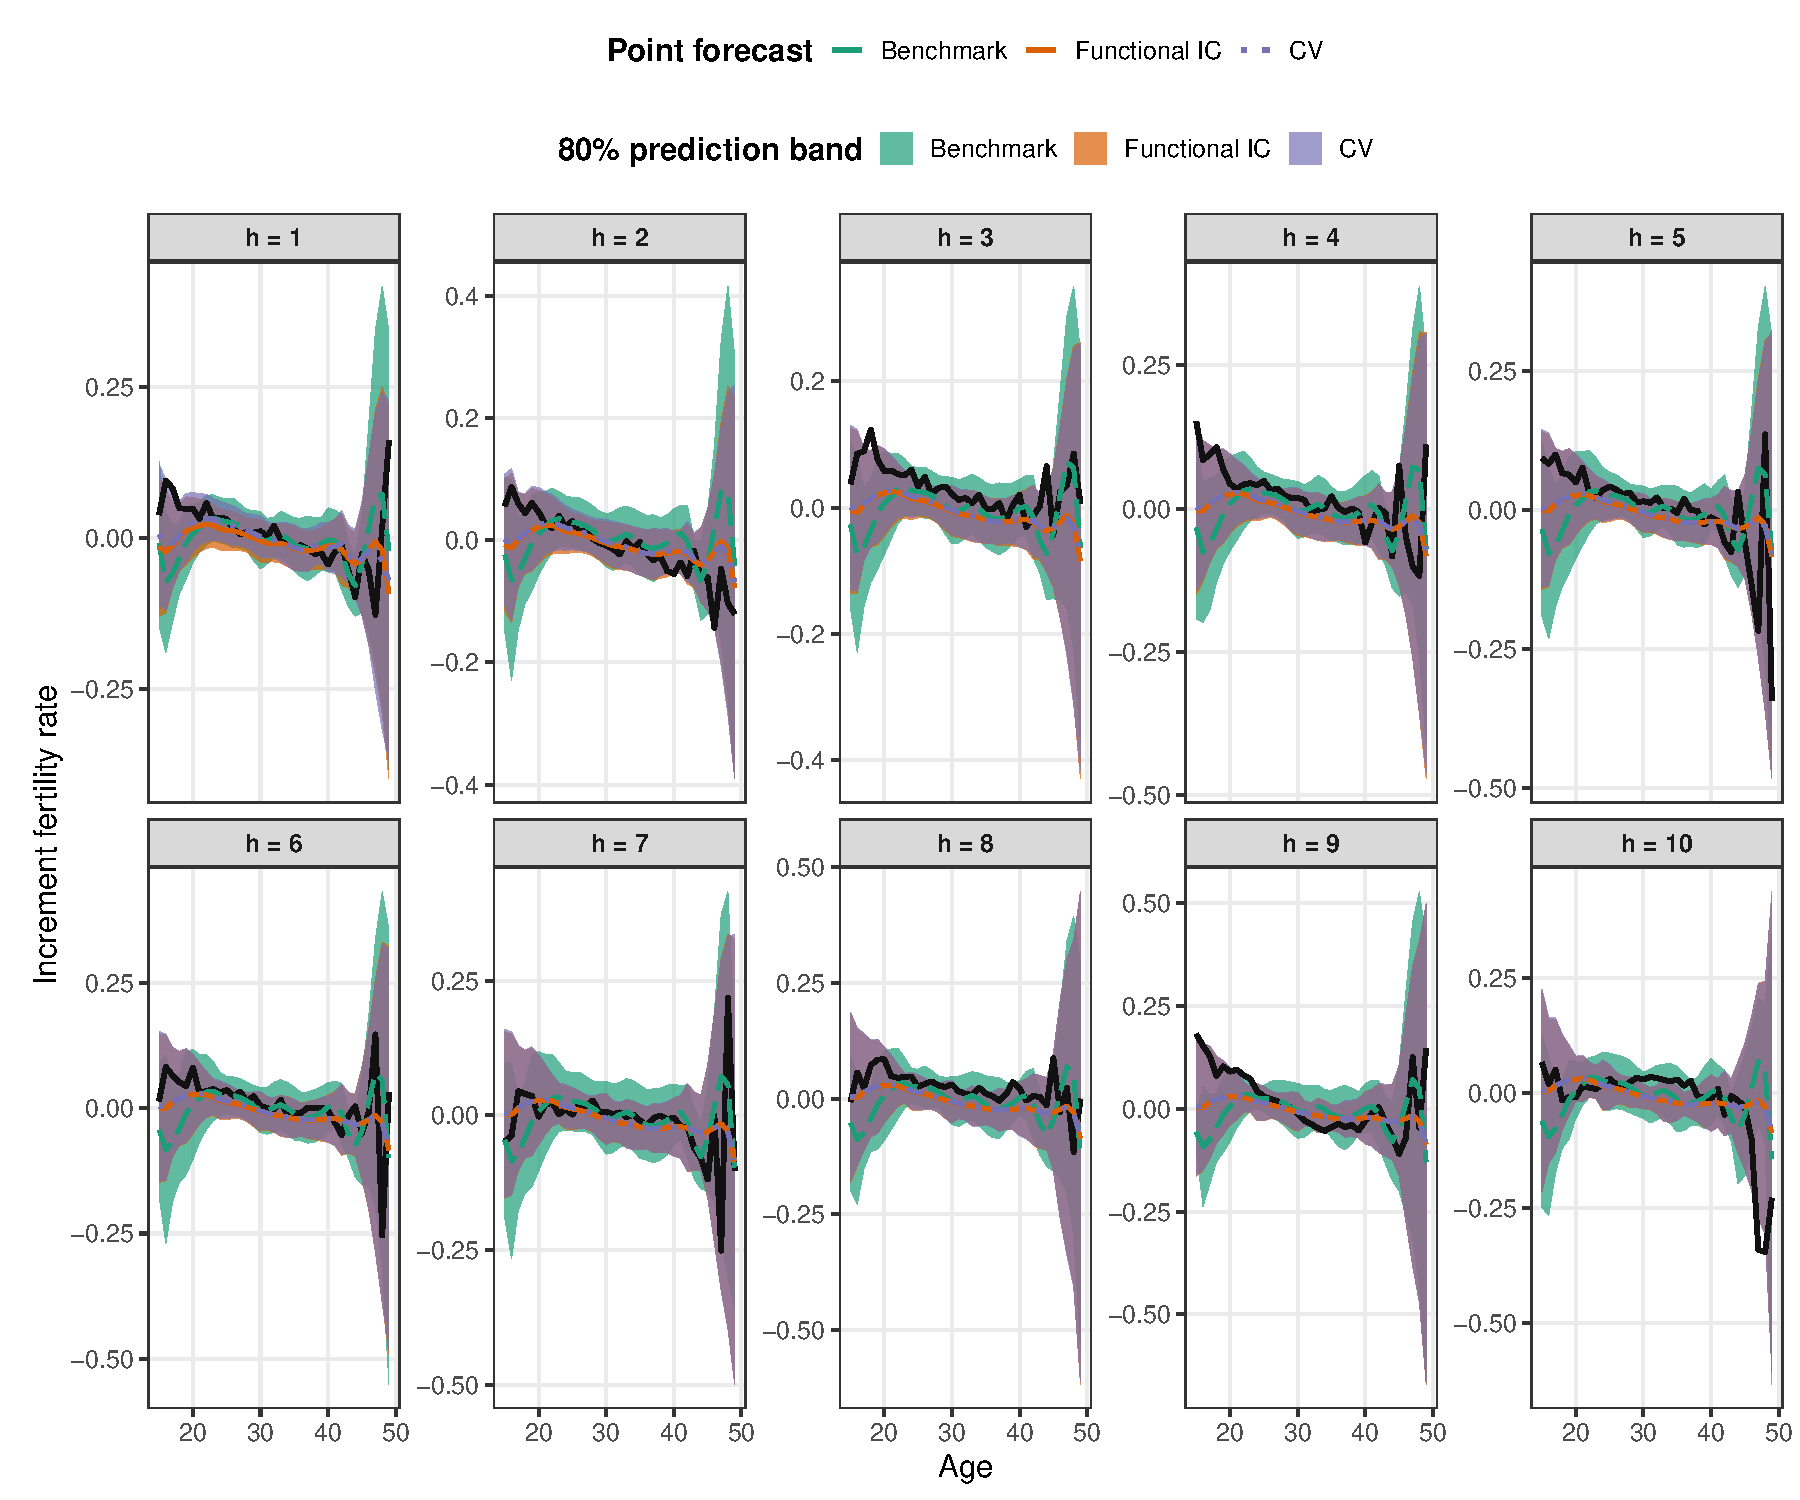
\includegraphics[width=0.98\textwidth]{Figures/Empirical/France_fertility_increment_forecasts_80.pdf}
\caption{\small French fertility-rate increment forecasts for horizons $h=1,\ldots,10$ at the latest common test origin. Black solid lines are raw observed curves. Coloured lines are point forecasts, and each central 80\% prediction band uses the colour of its corresponding method.}
\label{fig:emp-fertility-forecast}
\end{figure}

\clearpage
\subsection{French Female and Male Mortality}
\label{sec:emp-mortality}

\subsubsection{Data source and preprocessing}

The mortality data are annual age- and sex-specific death rates for the total population of France obtained from the Human Mortality Database \citep{HMD26}. The data, metadata, and download files are available from the \href{https://www.mortality.org/Country/Country?cntr=FRATNP}{Human Mortality Database France page}. The database constructs death rates from death counts and the corresponding exposures to risk \citep{Wilmoth25}. The sample covers 1861--2023 and contains 163 female and 163 male curves over ages 0--95.

Rates outside $(0,1]$ are treated as missing and linearly interpolated over time within each age. The analysis uses base-10 log-mortality rates. The raw curves are smoothed using weighted penalised regression splines, with exposure-based weights and a monotonicity constraint above age 65 following \citet{HU07}. Models are fitted to the smoothed curves, while RMSE, MAE, ECP, CPD, interval score, and WIS are evaluated against the raw log-mortality curves.

Figure~\ref{fig:emp-mortality-rainbow} shows the familiar mortality profile: high infant mortality, a rapid decline during childhood, and an approximately monotone increase through adulthood and old age. The progression from early red curves to recent violet curves reflects the substantial secular decline in mortality. Smoothing removes local age-specific variation while retaining the long-run shape and the more pronounced young-adult mortality hump for males.

\begin{figure}[!htb]
\centering
\includegraphics[width=0.88\textwidth]{Figures/Empirical/France_mortality_raw_smoothed.pdf}
\caption{\small Rainbow plots of raw and smoothed French female and male log-mortality rates, 1861--2023. The left column contains raw curves and the right column smoothed curves.}
\label{fig:emp-mortality-rainbow}
\end{figure}

Figure~\ref{fig:emp-mortality-facf} shows that the fACFs of both female and male log mortality decay slowly across the displayed lags, indicating strong long-range dependence. The stationarity test takes stationarity as its null hypothesis. The null is rejected for both series, with $p$-values of 0.0036 for females and 0.0040 for males, providing evidence that both log-mortality series are nonstationary.

\begin{figure}[!htb]
\centering
\begin{subfigure}[t]{0.48\textwidth}
\centering
\includegraphics[width=\textwidth]{Figures/Empirical/France_female_mortality_facf.pdf}
\caption{Female log mortality}
\end{subfigure}
\hfill
\begin{subfigure}[t]{0.48\textwidth}
\centering
\includegraphics[width=\textwidth]{Figures/Empirical/France_male_mortality_facf.pdf}
\caption{Male log mortality}
\end{subfigure}
\caption{\small Functional autocorrelation functions of French female and male log mortality. The dashed blue line is the simulated upper 95\% white-noise bound.}
\label{fig:emp-mortality-facf}
\end{figure}

\subsubsection{Forecasting results}

The BC-LPWN estimates are $\widehat d=0.9250$ for females and $0.9909$ for males. Both lie in the nonstationary fractional range $1/2<d<1$, and the male estimate is close to one. Conditional on these estimates, Functional IC selects $(p,q)=(0,1)$ for females and $(4,0)$ for males, whereas CV selects $(2,1)$ and $(2,3)$, respectively. The Functional IC results indicate a moving-average structure for females and an autoregressive structure with four lags for males. The selected short-memory orders therefore differ between the two series.

Figure~\ref{fig:emp-mortality-point-ratios} shows different results for female and male mortality. For females, the RMSE and MAE ratios of Functional IC and CV are below one at every horizon and are close to each other. The improvements are modest and vary across horizons. For males, the Functional IC ratios are also below one throughout, with improvements of approximately 1\%--5\%. In contrast, the CV ratios exceed one from $h=2$ onward. Functional IC therefore gives the most consistent point forecast performance for male mortality.

\begin{figure}[!htb]
\centering
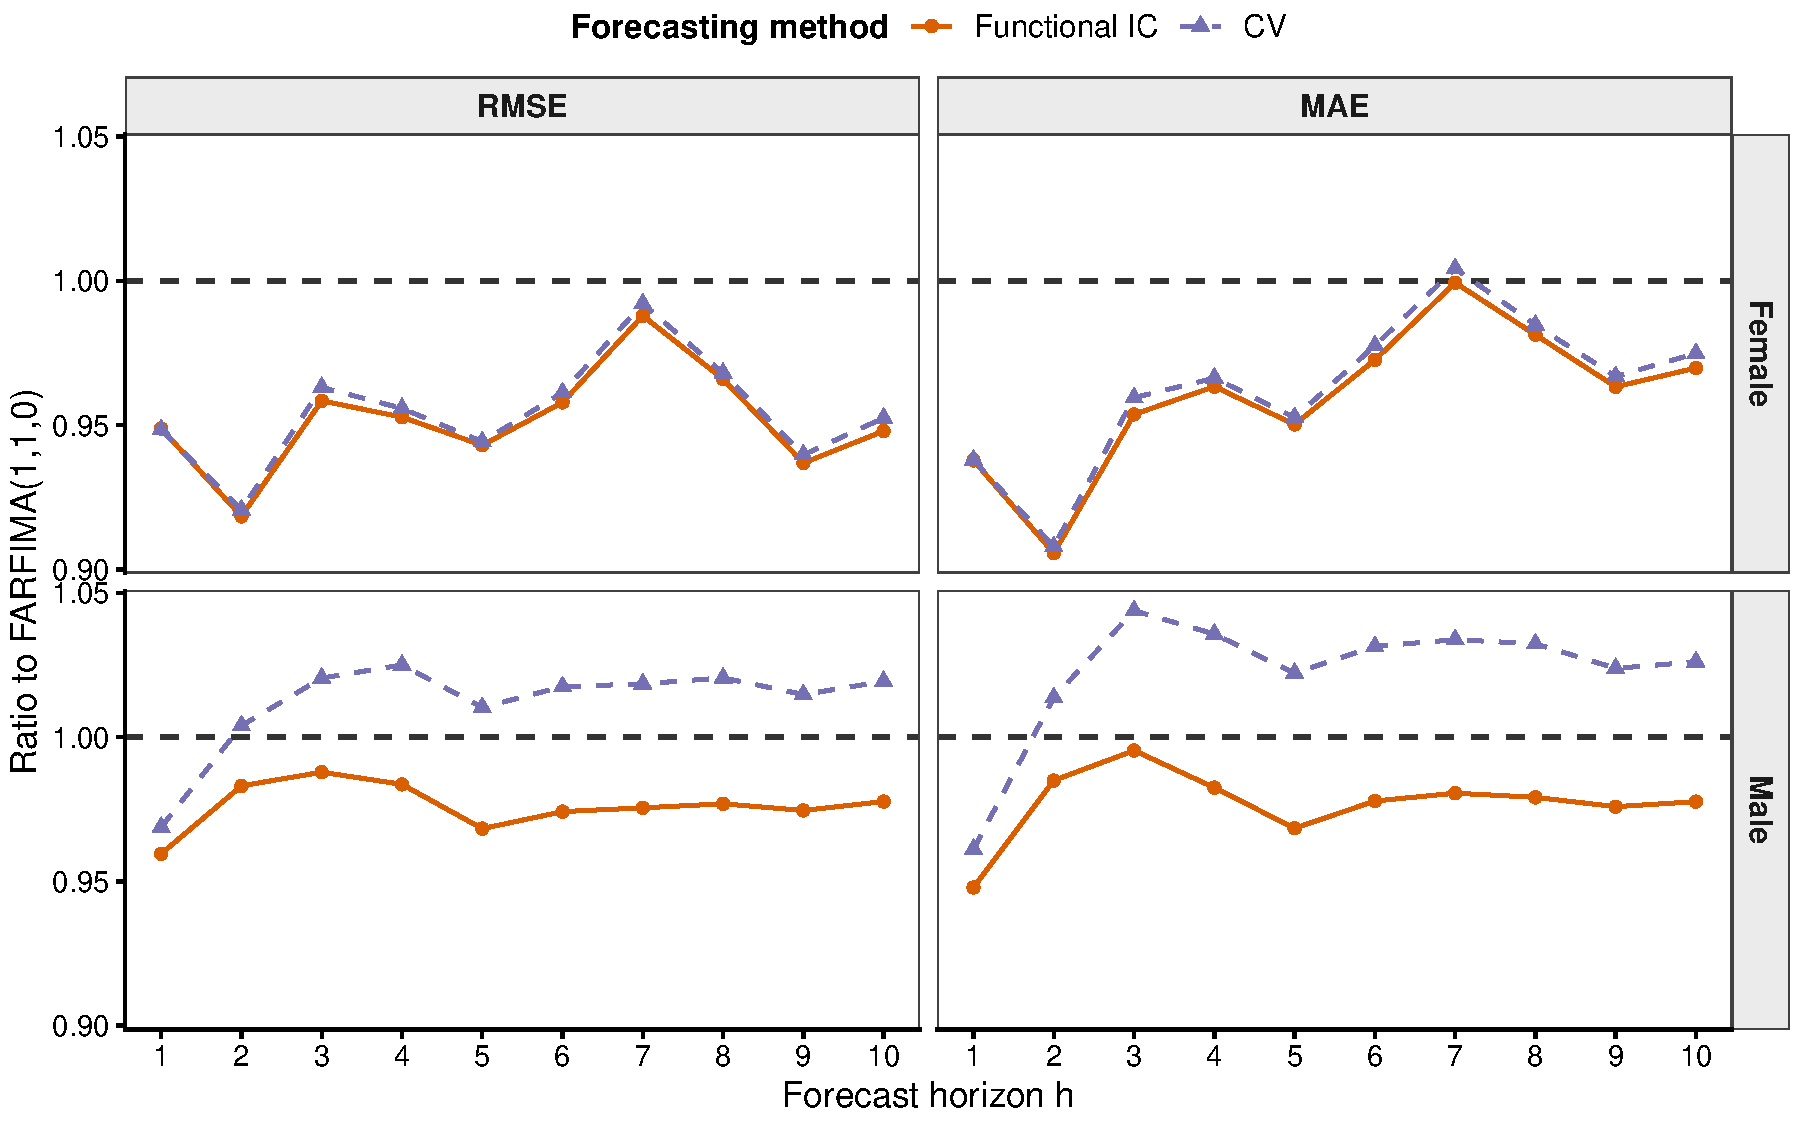
\includegraphics[width=0.98\textwidth]{Figures/Empirical/France_mortality_point_forecast_ratios.pdf}
\caption{\small RMSE and MAE ratios to FARFIMA$(1,1,0)$ for French female and male log mortality. Values below one indicate improvement over FARFIMA$(1,1,0)$.}
\label{fig:emp-mortality-point-ratios}
\end{figure}

Figure~\ref{fig:emp-mortality-ecp} shows the coverage results. Both sexes exhibit substantial under-coverage at short horizons. Coverage generally moves towards the nominal probabilities as the horizon increases, although the pattern is not monotone. The prediction bands are wider at longer horizons. In addition, the number of available forecast origins decreases from 25 at $h=1$ to 16 at $h=10$, so the longest-horizon estimates are more variable.

\begin{figure}[!htb]
\centering
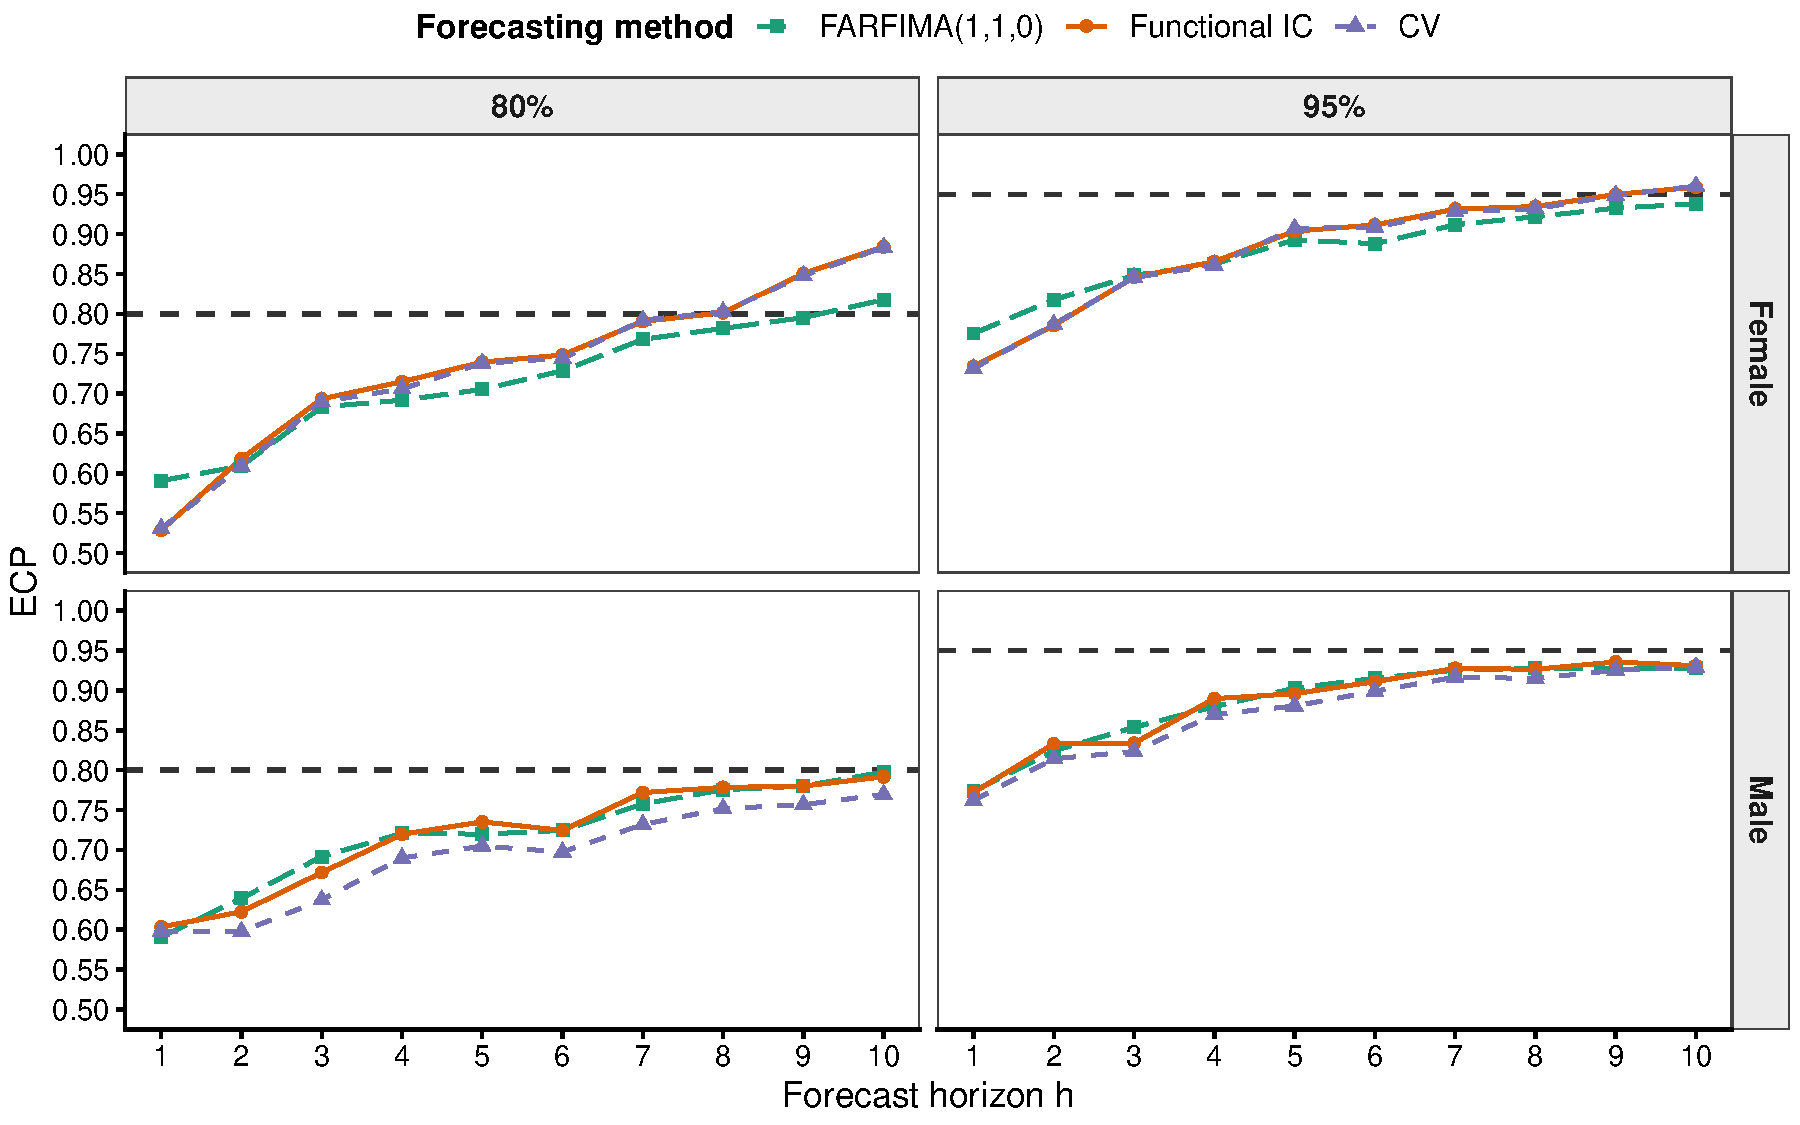
\includegraphics[width=0.98\textwidth]{Figures/Empirical/France_mortality_ecp.pdf}
\caption{\small Empirical coverage probabilities for the 80\% and 95\% prediction intervals for French female and male log mortality. Horizontal lines indicate the nominal coverage probabilities.}
\label{fig:emp-mortality-ecp}
\end{figure}

The interval score ratios in Figure~\ref{fig:emp-mortality-is-ratios} vary across horizons. For females, several short-horizon ratios exceed one, while most ratios from the middle horizons onward are below one. The weighted interval score ratios in Figure~\ref{fig:emp-mortality-wis-ratios} are below one from $h=2$ onward for both Functional IC and CV. For males, Functional IC generally gives interval score ratios below one and weighted interval score ratios below one at every horizon. The CV weighted interval score ratio exceeds one from $h=2$ onward. These results favour Functional IC for male interval forecasting. The score ratios should be interpreted together with the coverage results in Figure~\ref{fig:emp-mortality-ecp}.

\begin{figure}[!htb]
\centering
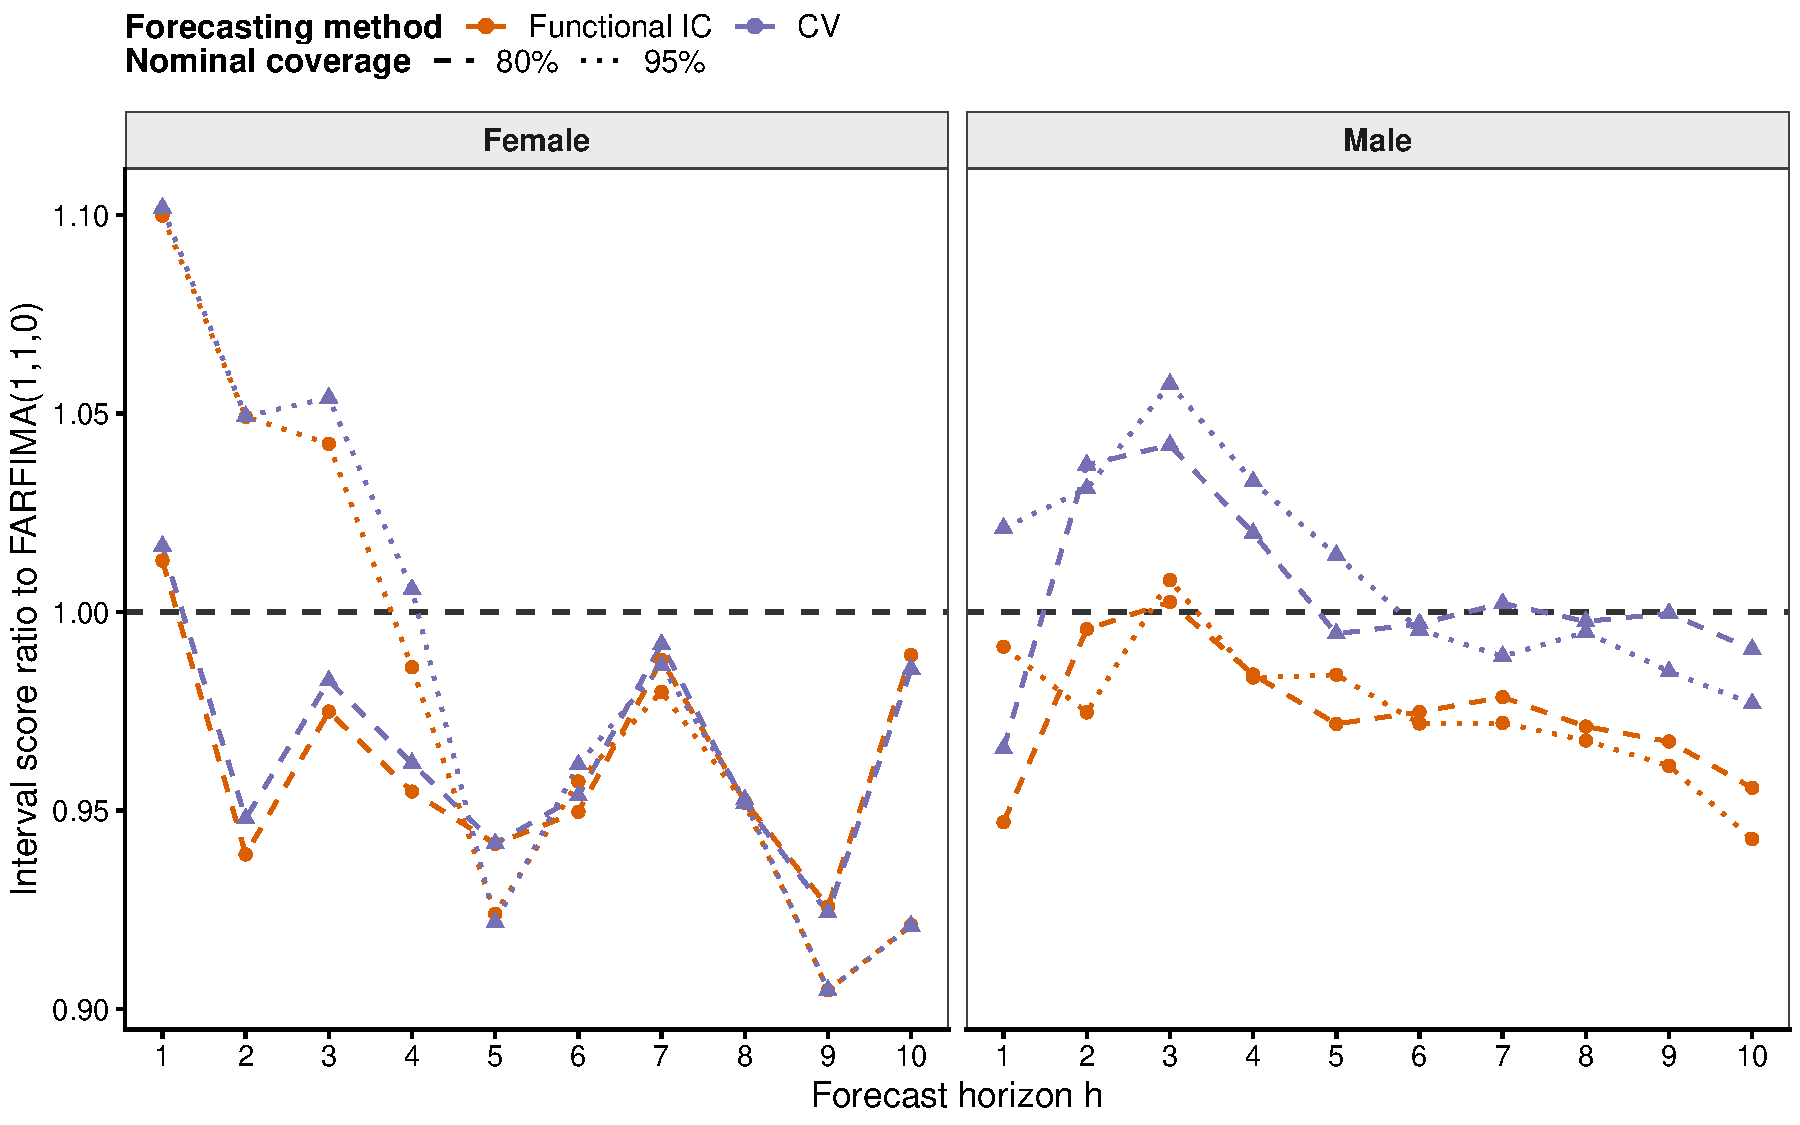
\includegraphics[width=0.98\textwidth]{Figures/Empirical/France_mortality_interval_score_ratios.pdf}
\caption{\small Interval Score Ratio to FARFIMA$(1,1,0)$ for French female and male log mortality. The 80\% and 95\% prediction intervals are distinguished by line type. Values below one indicate improvement over FARFIMA$(1,1,0)$.}
\label{fig:emp-mortality-is-ratios}
\end{figure}

\begin{figure}[!htb]
\centering
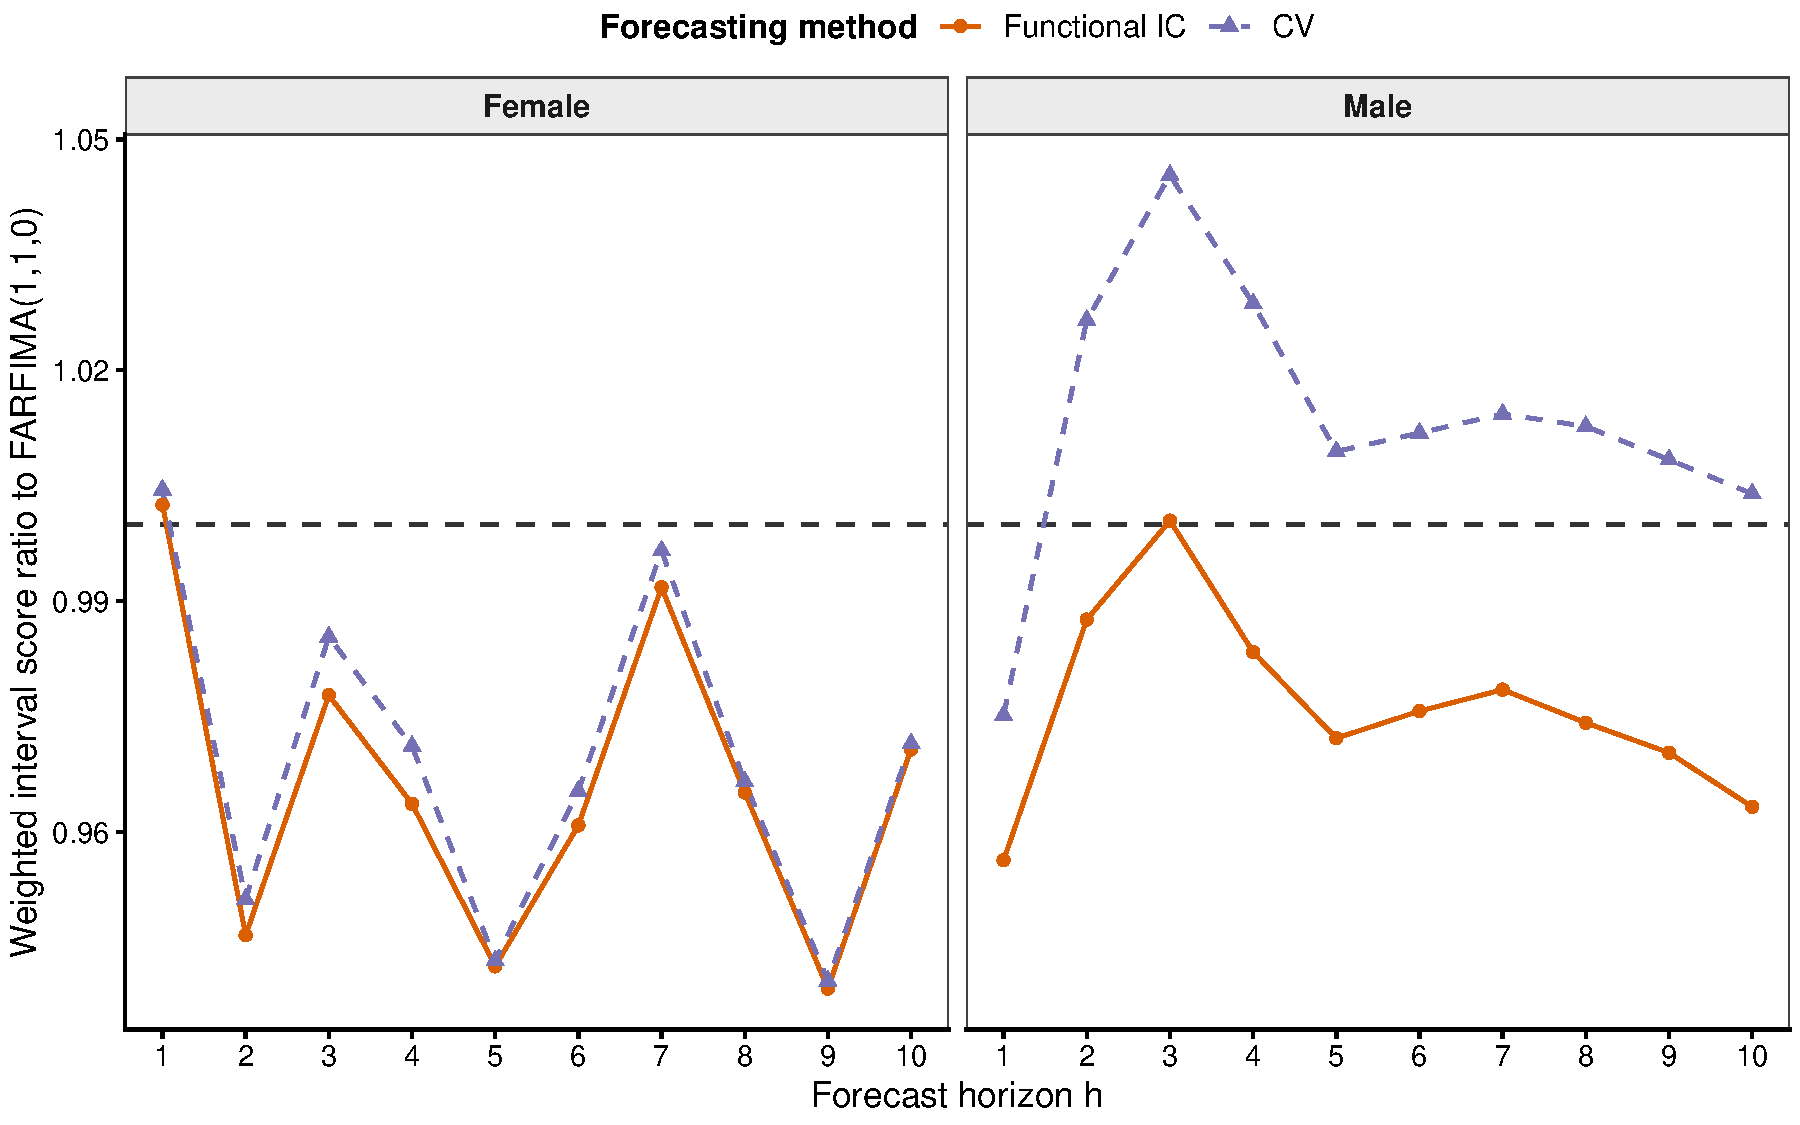
\includegraphics[width=0.98\textwidth]{Figures/Empirical/France_mortality_weighted_interval_score_ratios.pdf}
\caption{\small Weighted Interval Score Ratio to FARFIMA$(1,1,0)$ for French female and male log mortality. Values below one indicate improvement over FARFIMA$(1,1,0)$.}
\label{fig:emp-mortality-wis-ratios}
\end{figure}

\begin{small}
\setlength{\tabcolsep}{3pt}
\begin{longtable}[c]{crrrrrr}
\caption{\label{tab:emp-female-mortality-point}Point forecast accuracy for French female log mortality over all ten horizons. The smallest RMSE is red and the smallest MAE is blue.}\\
\toprule
 & \multicolumn{3}{c}{RMSE} & \multicolumn{3}{c}{MAE} \\
\cmidrule(lr){2-4} \cmidrule(lr){5-7}
$h$ & Bench. & IC & CV & Bench. & IC & CV \\
\midrule
\endfirsthead
\caption[]{Point forecast accuracy for French female log mortality over all ten horizons. The smallest RMSE is red and the smallest MAE is blue. \textit{(continued)}}\\
\toprule
 & \multicolumn{3}{c}{RMSE} & \multicolumn{3}{c}{MAE} \\
\cmidrule(lr){2-4} \cmidrule(lr){5-7}
$h$ & Bench. & IC & CV & Bench. & IC & CV \\
\midrule
\endhead

\endfoot
\bottomrule
\endlastfoot
1 & 0.0496 & \textcolor{red}{\textbf{0.0470}} & \textcolor{red}{\textbf{0.0470}} & 0.0317 & \textcolor{blue}{\textbf{0.0297}} & \textcolor{blue}{\textbf{0.0297}} \\
2 & 0.0537 & \textcolor{red}{\textbf{0.0493}} & 0.0494 & 0.0352 & \textcolor{blue}{\textbf{0.0318}} & 0.0319 \\
3 & 0.0533 & \textcolor{red}{\textbf{0.0511}} & 0.0513 & 0.0356 & \textcolor{blue}{\textbf{0.0340}} & 0.0342 \\
4 & 0.0549 & \textcolor{red}{\textbf{0.0523}} & 0.0525 & 0.0375 & \textcolor{blue}{\textbf{0.0362}} & 0.0363 \\
5 & 0.0591 & \textcolor{red}{\textbf{0.0557}} & 0.0558 & 0.0416 & \textcolor{blue}{\textbf{0.0396}} & 0.0397 \\
6 & 0.0609 & \textcolor{red}{\textbf{0.0583}} & 0.0585 & 0.0440 & \textcolor{blue}{\textbf{0.0427}} & 0.0430 \\
7 & 0.0615 & \textcolor{red}{\textbf{0.0607}} & 0.0610 & 0.0450 & \textcolor{blue}{\textbf{0.0449}} & 0.0452 \\
8 & 0.0662 & \textcolor{red}{\textbf{0.0640}} & 0.0641 & 0.0488 & \textcolor{blue}{\textbf{0.0479}} & 0.0481 \\
9 & 0.0703 & \textcolor{red}{\textbf{0.0659}} & 0.0661 & 0.0524 & \textcolor{blue}{\textbf{0.0504}} & 0.0506 \\
10 & 0.0699 & \textcolor{red}{\textbf{0.0663}} & 0.0666 & 0.0530 & \textcolor{blue}{\textbf{0.0514}} & 0.0517 \\
\end{longtable}
\end{small}


\begin{small}
\setlength{\tabcolsep}{3pt}
\begin{longtable}[c]{crrrrrr}
\caption{\label{tab:emp-male-mortality-point}Point forecast accuracy for French male log mortality over all ten horizons. The smallest RMSE is red and the smallest MAE is blue.}\\
\toprule
 & \multicolumn{3}{c}{RMSE} & \multicolumn{3}{c}{MAE} \\
\cmidrule(lr){2-4} \cmidrule(lr){5-7}
$h$ & Bench. & IC & CV & Bench. & IC & CV \\
\midrule
\endfirsthead
\caption[]{Point forecast accuracy for French male log mortality over all ten horizons. The smallest RMSE is red and the smallest MAE is blue. \textit{(continued)}}\\
\toprule
 & \multicolumn{3}{c}{RMSE} & \multicolumn{3}{c}{MAE} \\
\cmidrule(lr){2-4} \cmidrule(lr){5-7}
$h$ & Bench. & IC & CV & Bench. & IC & CV \\
\midrule
\endhead

\endfoot
\bottomrule
\endlastfoot
1 & 0.0385 & \textcolor{red}{\textbf{0.0369}} & 0.0373 & 0.0248 & \textcolor{blue}{\textbf{0.0235}} & 0.0238 \\
2 & 0.0409 & \textcolor{red}{\textbf{0.0402}} & 0.0411 & 0.0278 & \textcolor{blue}{\textbf{0.0274}} & 0.0282 \\
3 & 0.0439 & \textcolor{red}{\textbf{0.0434}} & 0.0448 & 0.0314 & \textcolor{blue}{\textbf{0.0312}} & 0.0327 \\
4 & 0.0476 & \textcolor{red}{\textbf{0.0468}} & 0.0488 & 0.0351 & \textcolor{blue}{\textbf{0.0345}} & 0.0364 \\
5 & 0.0530 & \textcolor{red}{\textbf{0.0513}} & 0.0535 & 0.0404 & \textcolor{blue}{\textbf{0.0391}} & 0.0413 \\
6 & 0.0582 & \textcolor{red}{\textbf{0.0567}} & 0.0592 & 0.0455 & \textcolor{blue}{\textbf{0.0445}} & 0.0469 \\
7 & 0.0628 & \textcolor{red}{\textbf{0.0613}} & 0.0640 & 0.0494 & \textcolor{blue}{\textbf{0.0484}} & 0.0510 \\
8 & 0.0671 & \textcolor{red}{\textbf{0.0655}} & 0.0685 & 0.0535 & \textcolor{blue}{\textbf{0.0524}} & 0.0552 \\
9 & 0.0725 & \textcolor{red}{\textbf{0.0706}} & 0.0735 & 0.0584 & \textcolor{blue}{\textbf{0.0570}} & 0.0598 \\
10 & 0.0765 & \textcolor{red}{\textbf{0.0748}} & 0.0780 & 0.0619 & \textcolor{blue}{\textbf{0.0605}} & 0.0635 \\
\end{longtable}
\end{small}


\begingroup
\setlength{\tabcolsep}{3pt}
\setlength{\LTleft}{\fill}
\setlength{\LTright}{\fill}
\begingroup\fontsize{7}{9}\selectfont
\begin{longtable}[c]{ccrrrrrrrrr}
\caption{Interval forecast performance for French female log mortality over all ten horizons. The smallest CPD is red and the smallest interval score is blue.}\label{tab:emp-female-mortality-interval}\\
\toprule
 & & \multicolumn{3}{c}{ECP} & \multicolumn{3}{c}{CPD} & \multicolumn{3}{c}{Score} \\
\cmidrule(lr){3-5} \cmidrule(lr){6-8} \cmidrule(lr){9-11}
$h$ & CP & Bench. & IC & CV & Bench. & IC & CV & Bench. & IC & CV \\
\midrule
\endfirsthead
\caption[]{Interval forecast performance for French female log mortality over all ten horizons. The smallest CPD is red and the smallest interval score is blue. \textit{(continued)}}\\
\toprule
 & & \multicolumn{3}{c}{ECP} & \multicolumn{3}{c}{CPD} & \multicolumn{3}{c}{Score} \\
\cmidrule(lr){3-5} \cmidrule(lr){6-8} \cmidrule(lr){9-11}
$h$ & CP & Bench. & IC & CV & Bench. & IC & CV & Bench. & IC & CV \\
\midrule
\endhead

\endfoot
\bottomrule
\endlastfoot
1 & 95\% & 0.7754 & 0.7342 & 0.7317 & \textcolor{red}{\textbf{0.1746}} & 0.2158 & 0.2183 & \textcolor{blue}{\textbf{0.3478}} & 0.3825 & 0.3832 \\
 & 80\% & 0.5908 & 0.5288 & 0.5308 & \textcolor{red}{\textbf{0.2092}} & 0.2712 & 0.2692 & \textcolor{blue}{\textbf{0.1717}} & 0.1739 & 0.1745 \\
\cmidrule(lr){1-11}
2 & 95\% & 0.8177 & 0.7856 & 0.7869 & \textcolor{red}{\textbf{0.1323}} & 0.1644 & 0.1631 & \textcolor{blue}{\textbf{0.3362}} & 0.3528 & 0.3528 \\
 & 80\% & 0.6094 & 0.6185 & 0.6089 & 0.1906 & \textcolor{red}{\textbf{0.1815}} & 0.1911 & 0.1853 & \textcolor{blue}{\textbf{0.1740}} & 0.1757 \\
\cmidrule(lr){1-11}
3 & 95\% & 0.8483 & 0.8460 & 0.8456 & \textcolor{red}{\textbf{0.1017}} & 0.1040 & 0.1044 & \textcolor{blue}{\textbf{0.2960}} & 0.3086 & 0.3120 \\
 & 80\% & 0.6834 & 0.6934 & 0.6898 & 0.1166 & \textcolor{red}{\textbf{0.1066}} & 0.1102 & 0.1749 & \textcolor{blue}{\textbf{0.1706}} & 0.1719 \\
\cmidrule(lr){1-11}
4 & 95\% & 0.8627 & 0.8655 & 0.8613 & 0.0873 & \textcolor{red}{\textbf{0.0845}} & 0.0887 & 0.3028 & \textcolor{blue}{\textbf{0.2986}} & 0.3045 \\
 & 80\% & 0.6918 & 0.7150 & 0.7060 & 0.1082 & \textcolor{red}{\textbf{0.0850}} & 0.0940 & 0.1841 & \textcolor{blue}{\textbf{0.1758}} & 0.1771 \\
\cmidrule(lr){1-11}
5 & 95\% & 0.8929 & 0.9038 & 0.9072 & 0.0571 & 0.0462 & \textcolor{red}{\textbf{0.0428}} & 0.3032 & 0.2802 & \textcolor{blue}{\textbf{0.2796}} \\
 & 80\% & 0.7054 & 0.7396 & 0.7381 & 0.0946 & \textcolor{red}{\textbf{0.0604}} & 0.0619 & 0.1967 & \textcolor{blue}{\textbf{0.1852}} & \textcolor{blue}{\textbf{0.1852}} \\
\cmidrule(lr){1-11}
6 & 95\% & 0.8880 & 0.9115 & 0.9089 & 0.0620 & \textcolor{red}{\textbf{0.0385}} & 0.0411 & 0.3114 & \textcolor{blue}{\textbf{0.2981}} & 0.2995 \\
 & 80\% & 0.7286 & 0.7484 & 0.7443 & 0.0714 & \textcolor{red}{\textbf{0.0516}} & 0.0557 & 0.2049 & \textcolor{blue}{\textbf{0.1946}} & 0.1955 \\
\cmidrule(lr){1-11}
7 & 95\% & 0.9117 & 0.9315 & 0.9282 & 0.0383 & \textcolor{red}{\textbf{0.0185}} & 0.0218 & 0.3047 & \textcolor{blue}{\textbf{0.2986}} & 0.3006 \\
 & 80\% & 0.7681 & 0.7906 & 0.7922 & 0.0319 & 0.0094 & \textcolor{red}{\textbf{0.0078}} & 0.2064 & \textcolor{blue}{\textbf{0.2039}} & 0.2047 \\
\cmidrule(lr){1-11}
8 & 95\% & 0.9219 & 0.9346 & 0.9317 & 0.0281 & \textcolor{red}{\textbf{0.0154}} & 0.0183 & 0.3179 & \textcolor{blue}{\textbf{0.3027}} & 0.3029 \\
 & 80\% & 0.7818 & 0.8015 & 0.8027 & 0.0182 & \textcolor{red}{\textbf{0.0015}} & 0.0027 & 0.2255 & 0.2148 & \textcolor{blue}{\textbf{0.2147}} \\
\cmidrule(lr){1-11}
9 & 95\% & 0.9326 & 0.9498 & 0.9485 & 0.0174 & \textcolor{red}{\textbf{0.0002}} & 0.0015 & 0.3304 & \textcolor{blue}{\textbf{0.2990}} & \textcolor{blue}{\textbf{0.2990}} \\
 & 80\% & 0.7953 & 0.8505 & 0.8480 & \textcolor{red}{\textbf{0.0047}} & 0.0505 & 0.0480 & 0.2378 & 0.2202 & \textcolor{blue}{\textbf{0.2198}} \\
\cmidrule(lr){1-11}
10 & 95\% & 0.9382 & 0.9590 & 0.9603 & 0.0118 & \textcolor{red}{\textbf{0.0090}} & 0.0103 & 0.3527 & 0.3249 & \textcolor{blue}{\textbf{0.3248}} \\
 & 80\% & 0.8177 & 0.8841 & 0.8835 & \textcolor{red}{\textbf{0.0177}} & 0.0841 & 0.0835 & 0.2512 & 0.2485 & \textcolor{blue}{\textbf{0.2476}} \\
\end{longtable}
\endgroup
\endgroup

\begin{table}[!htb]
\centering
\begingroup\fontsize{7}{9}\selectfont
\setlength{\tabcolsep}{2.5pt}
\caption{Weighted interval score for French female log mortality over all ten horizons. The smallest WIS at each horizon is highlighted in purple.}
\label{tab:emp-female-mortality-wis}
\begin{tabular}{lrrrrrrrrrr}
\toprule
Method & $h=1$ & $h=2$ & $h=3$ & $h=4$ & $h=5$ & $h=6$ & $h=7$ & $h=8$ & $h=9$ & $h=10$ \\
\midrule
FARFIMA$(1,1,0)$ & \textcolor{purple}{\textbf{0.0167}} & 0.0178 & 0.0171 & 0.0179 & 0.0192 & 0.0201 & 0.0203 & 0.0220 & 0.0233 & 0.0242 \\
Functional IC & \textcolor{purple}{\textbf{0.0167}} & \textcolor{purple}{\textbf{0.0169}} & \textcolor{purple}{\textbf{0.0167}} & \textcolor{purple}{\textbf{0.0172}} & \textcolor{purple}{\textbf{0.0181}} & \textcolor{purple}{\textbf{0.0193}} & \textcolor{purple}{\textbf{0.0201}} & \textcolor{purple}{\textbf{0.0212}} & \textcolor{purple}{\textbf{0.0219}} & \textcolor{purple}{\textbf{0.0235}} \\
CV & 0.0168 & \textcolor{purple}{\textbf{0.0169}} & 0.0168 & 0.0174 & \textcolor{purple}{\textbf{0.0181}} & 0.0194 & 0.0202 & \textcolor{purple}{\textbf{0.0212}} & \textcolor{purple}{\textbf{0.0219}} & \textcolor{purple}{\textbf{0.0235}} \\
\bottomrule
\end{tabular}
\endgroup
\end{table}


\begingroup
\setlength{\tabcolsep}{3pt}
\setlength{\LTleft}{\fill}
\setlength{\LTright}{\fill}
\begingroup\fontsize{7}{9}\selectfont
\begin{longtable}[c]{ccrrrrrrrrr}
\caption{Interval forecast performance for French male log mortality over all ten horizons. The smallest CPD is red and the smallest interval score is blue.}\label{tab:emp-male-mortality-interval}\\
\toprule
 & & \multicolumn{3}{c}{ECP} & \multicolumn{3}{c}{CPD} & \multicolumn{3}{c}{Score} \\
\cmidrule(lr){3-5} \cmidrule(lr){6-8} \cmidrule(lr){9-11}
$h$ & CP & Bench. & IC & CV & Bench. & IC & CV & Bench. & IC & CV \\
\midrule
\endfirsthead
\caption[]{Interval forecast performance for French male log mortality over all ten horizons. The smallest CPD is red and the smallest interval score is blue. \textit{(continued)}}\\
\toprule
 & & \multicolumn{3}{c}{ECP} & \multicolumn{3}{c}{CPD} & \multicolumn{3}{c}{Score} \\
\cmidrule(lr){3-5} \cmidrule(lr){6-8} \cmidrule(lr){9-11}
$h$ & CP & Bench. & IC & CV & Bench. & IC & CV & Bench. & IC & CV \\
\midrule
\endhead

\endfoot
\bottomrule
\endlastfoot
1 & 95\% & 0.7738 & 0.7721 & 0.7621 & \textcolor{red}{\textbf{0.1762}} & 0.1779 & 0.1879 & 0.2631 & \textcolor{blue}{\textbf{0.2608}} & 0.2687 \\
 & 80\% & 0.5908 & 0.6033 & 0.5983 & 0.2092 & \textcolor{red}{\textbf{0.1967}} & 0.2017 & 0.1347 & \textcolor{blue}{\textbf{0.1276}} & 0.1301 \\
\cmidrule(lr){1-11}
2 & 95\% & 0.8242 & 0.8329 & 0.8142 & 0.1258 & \textcolor{red}{\textbf{0.1171}} & 0.1358 & 0.2420 & \textcolor{blue}{\textbf{0.2359}} & 0.2495 \\
 & 80\% & 0.6393 & 0.6224 & 0.5977 & \textcolor{red}{\textbf{0.1607}} & 0.1776 & 0.2023 & 0.1421 & \textcolor{blue}{\textbf{0.1415}} & 0.1474 \\
\cmidrule(lr){1-11}
3 & 95\% & 0.8537 & 0.8338 & 0.8234 & \textcolor{red}{\textbf{0.0963}} & 0.1162 & 0.1266 & \textcolor{blue}{\textbf{0.2484}} & 0.2504 & 0.2626 \\
 & 80\% & 0.6916 & 0.6716 & 0.6372 & \textcolor{red}{\textbf{0.1084}} & 0.1284 & 0.1628 & \textcolor{blue}{\textbf{0.1568}} & 0.1572 & 0.1634 \\
\cmidrule(lr){1-11}
4 & 95\% & 0.8797 & 0.8897 & 0.8698 & 0.0703 & \textcolor{red}{\textbf{0.0603}} & 0.0802 & 0.2555 & \textcolor{blue}{\textbf{0.2512}} & 0.2639 \\
 & 80\% & 0.7206 & 0.7197 & 0.6899 & \textcolor{red}{\textbf{0.0794}} & 0.0803 & 0.1101 & 0.1709 & \textcolor{blue}{\textbf{0.1682}} & 0.1743 \\
\cmidrule(lr){1-11}
5 & 95\% & 0.9028 & 0.8958 & 0.8805 & \textcolor{red}{\textbf{0.0472}} & 0.0542 & 0.0695 & 0.2798 & \textcolor{blue}{\textbf{0.2754}} & 0.2839 \\
 & 80\% & 0.7197 & 0.7351 & 0.7049 & 0.0803 & \textcolor{red}{\textbf{0.0649}} & 0.0951 & 0.1950 & \textcolor{blue}{\textbf{0.1895}} & 0.1939 \\
\cmidrule(lr){1-11}
6 & 95\% & 0.9151 & 0.9109 & 0.8990 & \textcolor{red}{\textbf{0.0349}} & 0.0391 & 0.0510 & 0.3130 & \textcolor{blue}{\textbf{0.3042}} & 0.3116 \\
 & 80\% & 0.7245 & 0.7245 & 0.6974 & \textcolor{red}{\textbf{0.0755}} & \textcolor{red}{\textbf{0.0755}} & 0.1026 & 0.2147 & \textcolor{blue}{\textbf{0.2093}} & 0.2141 \\
\cmidrule(lr){1-11}
7 & 95\% & 0.9254 & 0.9276 & 0.9167 & 0.0246 & \textcolor{red}{\textbf{0.0224}} & 0.0333 & 0.3232 & \textcolor{blue}{\textbf{0.3142}} & 0.3196 \\
 & 80\% & 0.7577 & 0.7719 & 0.7319 & 0.0423 & \textcolor{red}{\textbf{0.0281}} & 0.0681 & 0.2264 & \textcolor{blue}{\textbf{0.2215}} & 0.2268 \\
\cmidrule(lr){1-11}
8 & 95\% & 0.9277 & 0.9265 & 0.9149 & \textcolor{red}{\textbf{0.0223}} & 0.0235 & 0.0351 & 0.3491 & \textcolor{blue}{\textbf{0.3378}} & 0.3473 \\
 & 80\% & 0.7755 & 0.7784 & 0.7517 & 0.0245 & \textcolor{red}{\textbf{0.0216}} & 0.0483 & 0.2460 & \textcolor{blue}{\textbf{0.2389}} & 0.2454 \\
\cmidrule(lr){1-11}
9 & 95\% & 0.9277 & 0.9357 & 0.9252 & 0.0223 & \textcolor{red}{\textbf{0.0143}} & 0.0248 & 0.3780 & \textcolor{blue}{\textbf{0.3634}} & 0.3724 \\
 & 80\% & 0.7800 & 0.7800 & 0.7567 & \textcolor{red}{\textbf{0.0200}} & \textcolor{red}{\textbf{0.0200}} & 0.0433 & 0.2644 & \textcolor{blue}{\textbf{0.2557}} & 0.2643 \\
\cmidrule(lr){1-11}
10 & 95\% & 0.9277 & 0.9310 & 0.9290 & 0.0223 & \textcolor{red}{\textbf{0.0190}} & 0.0210 & 0.4281 & \textcolor{blue}{\textbf{0.4037}} & 0.4183 \\
 & 80\% & 0.7975 & 0.7917 & 0.7695 & \textcolor{red}{\textbf{0.0025}} & 0.0083 & 0.0305 & 0.2963 & \textcolor{blue}{\textbf{0.2832}} & 0.2935 \\
\end{longtable}
\endgroup
\endgroup

\begin{table}[!htb]
\centering
\begingroup\fontsize{7}{9}\selectfont
\setlength{\tabcolsep}{2.5pt}
\caption{Weighted interval score for French male log mortality over all ten horizons. The smallest WIS at each horizon is highlighted in purple.}
\label{tab:emp-male-mortality-wis}
\begin{tabular}{lrrrrrrrrrr}
\toprule
Method & $h=1$ & $h=2$ & $h=3$ & $h=4$ & $h=5$ & $h=6$ & $h=7$ & $h=8$ & $h=9$ & $h=10$ \\
\midrule
FARFIMA$(1,1,0)$ & 0.0130 & 0.0137 & \textcolor{purple}{\textbf{0.0150}} & 0.0164 & 0.0187 & 0.0208 & 0.0222 & 0.0240 & 0.0260 & 0.0285 \\
Functional IC & \textcolor{purple}{\textbf{0.0124}} & \textcolor{purple}{\textbf{0.0135}} & \textcolor{purple}{\textbf{0.0150}} & \textcolor{purple}{\textbf{0.0161}} & \textcolor{purple}{\textbf{0.0182}} & \textcolor{purple}{\textbf{0.0203}} & \textcolor{purple}{\textbf{0.0217}} & \textcolor{purple}{\textbf{0.0234}} & \textcolor{purple}{\textbf{0.0253}} & \textcolor{purple}{\textbf{0.0275}} \\
CV & 0.0127 & 0.0140 & 0.0157 & 0.0169 & 0.0189 & 0.0211 & 0.0225 & 0.0243 & 0.0262 & 0.0286 \\
\bottomrule
\end{tabular}
\endgroup
\end{table}

For reference, Tables~\ref{tab:emp-female-mortality-point}--\ref{tab:emp-male-mortality-wis} report the metric values before division by the FARFIMA$(1,1,0)$ benchmark. They provide the numerical results corresponding to the ratio figures.


Figures~\ref{fig:emp-female-mortality-forecast} and \ref{fig:emp-male-mortality-forecast} present forecasts for all horizons $h=1,\ldots,10$ at the latest common test origin. The three methods produce similar forecast curves for females. Differences are more visible for males at the longer horizons. The ratio figures show that Functional IC gives the most consistent performance, particularly for male mortality.

\begin{figure}[!htb]
\centering
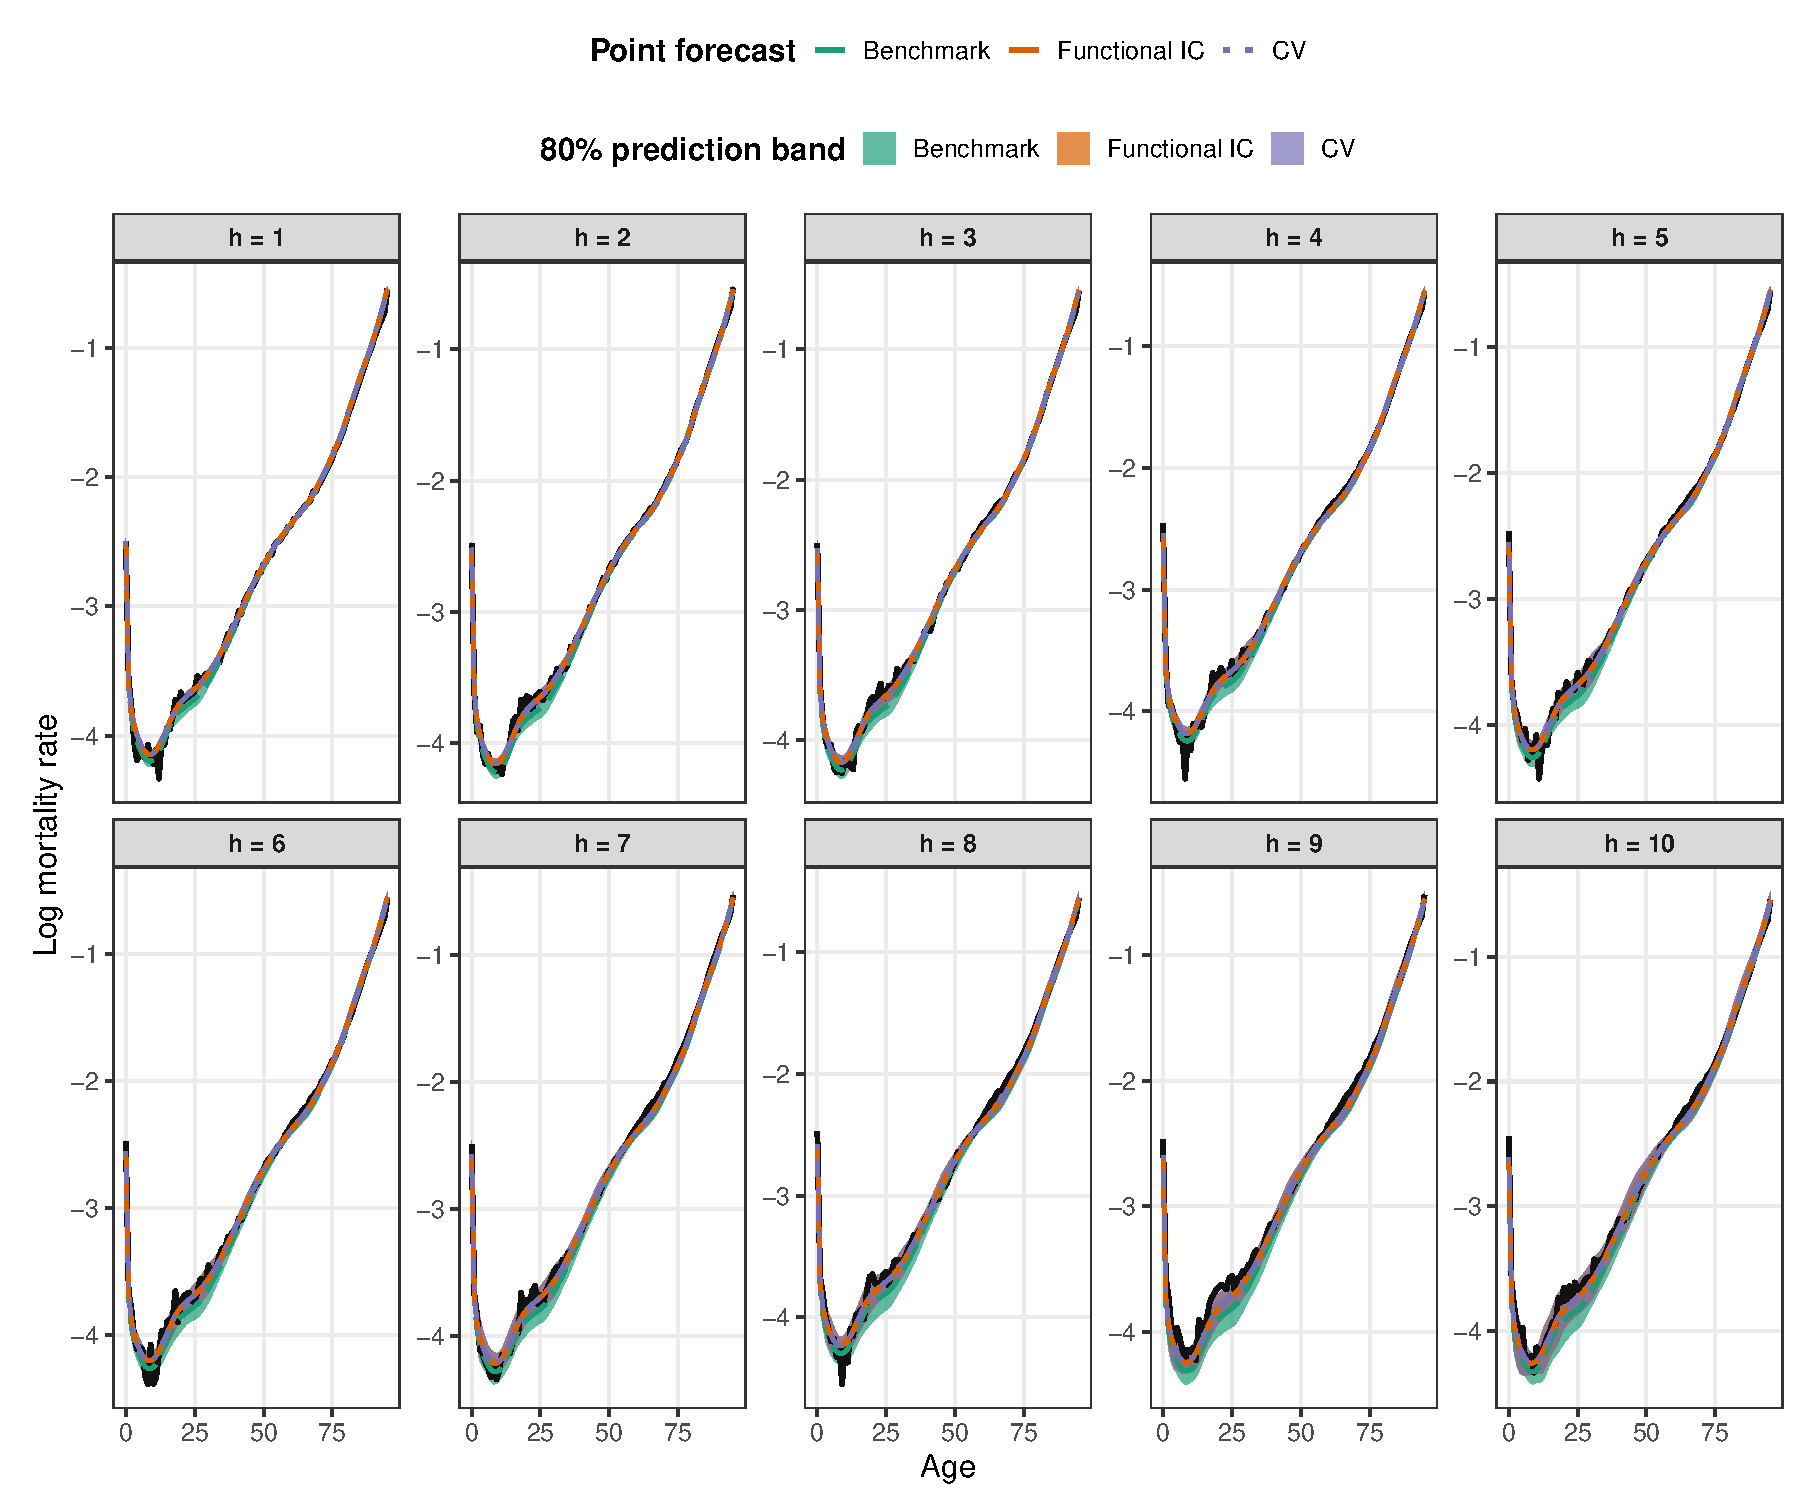
\includegraphics[width=0.98\textwidth]{Figures/Empirical/France_female_mortality_forecasts_80.pdf}
\caption{\small French female log-mortality forecasts for horizons $h=1,\ldots,10$ at the latest common test origin. Black solid lines are raw observed curves. Coloured lines are point forecasts, and each central 80\% prediction band uses the colour of its corresponding method.}
\label{fig:emp-female-mortality-forecast}
\end{figure}

\begin{figure}[!htb]
\centering
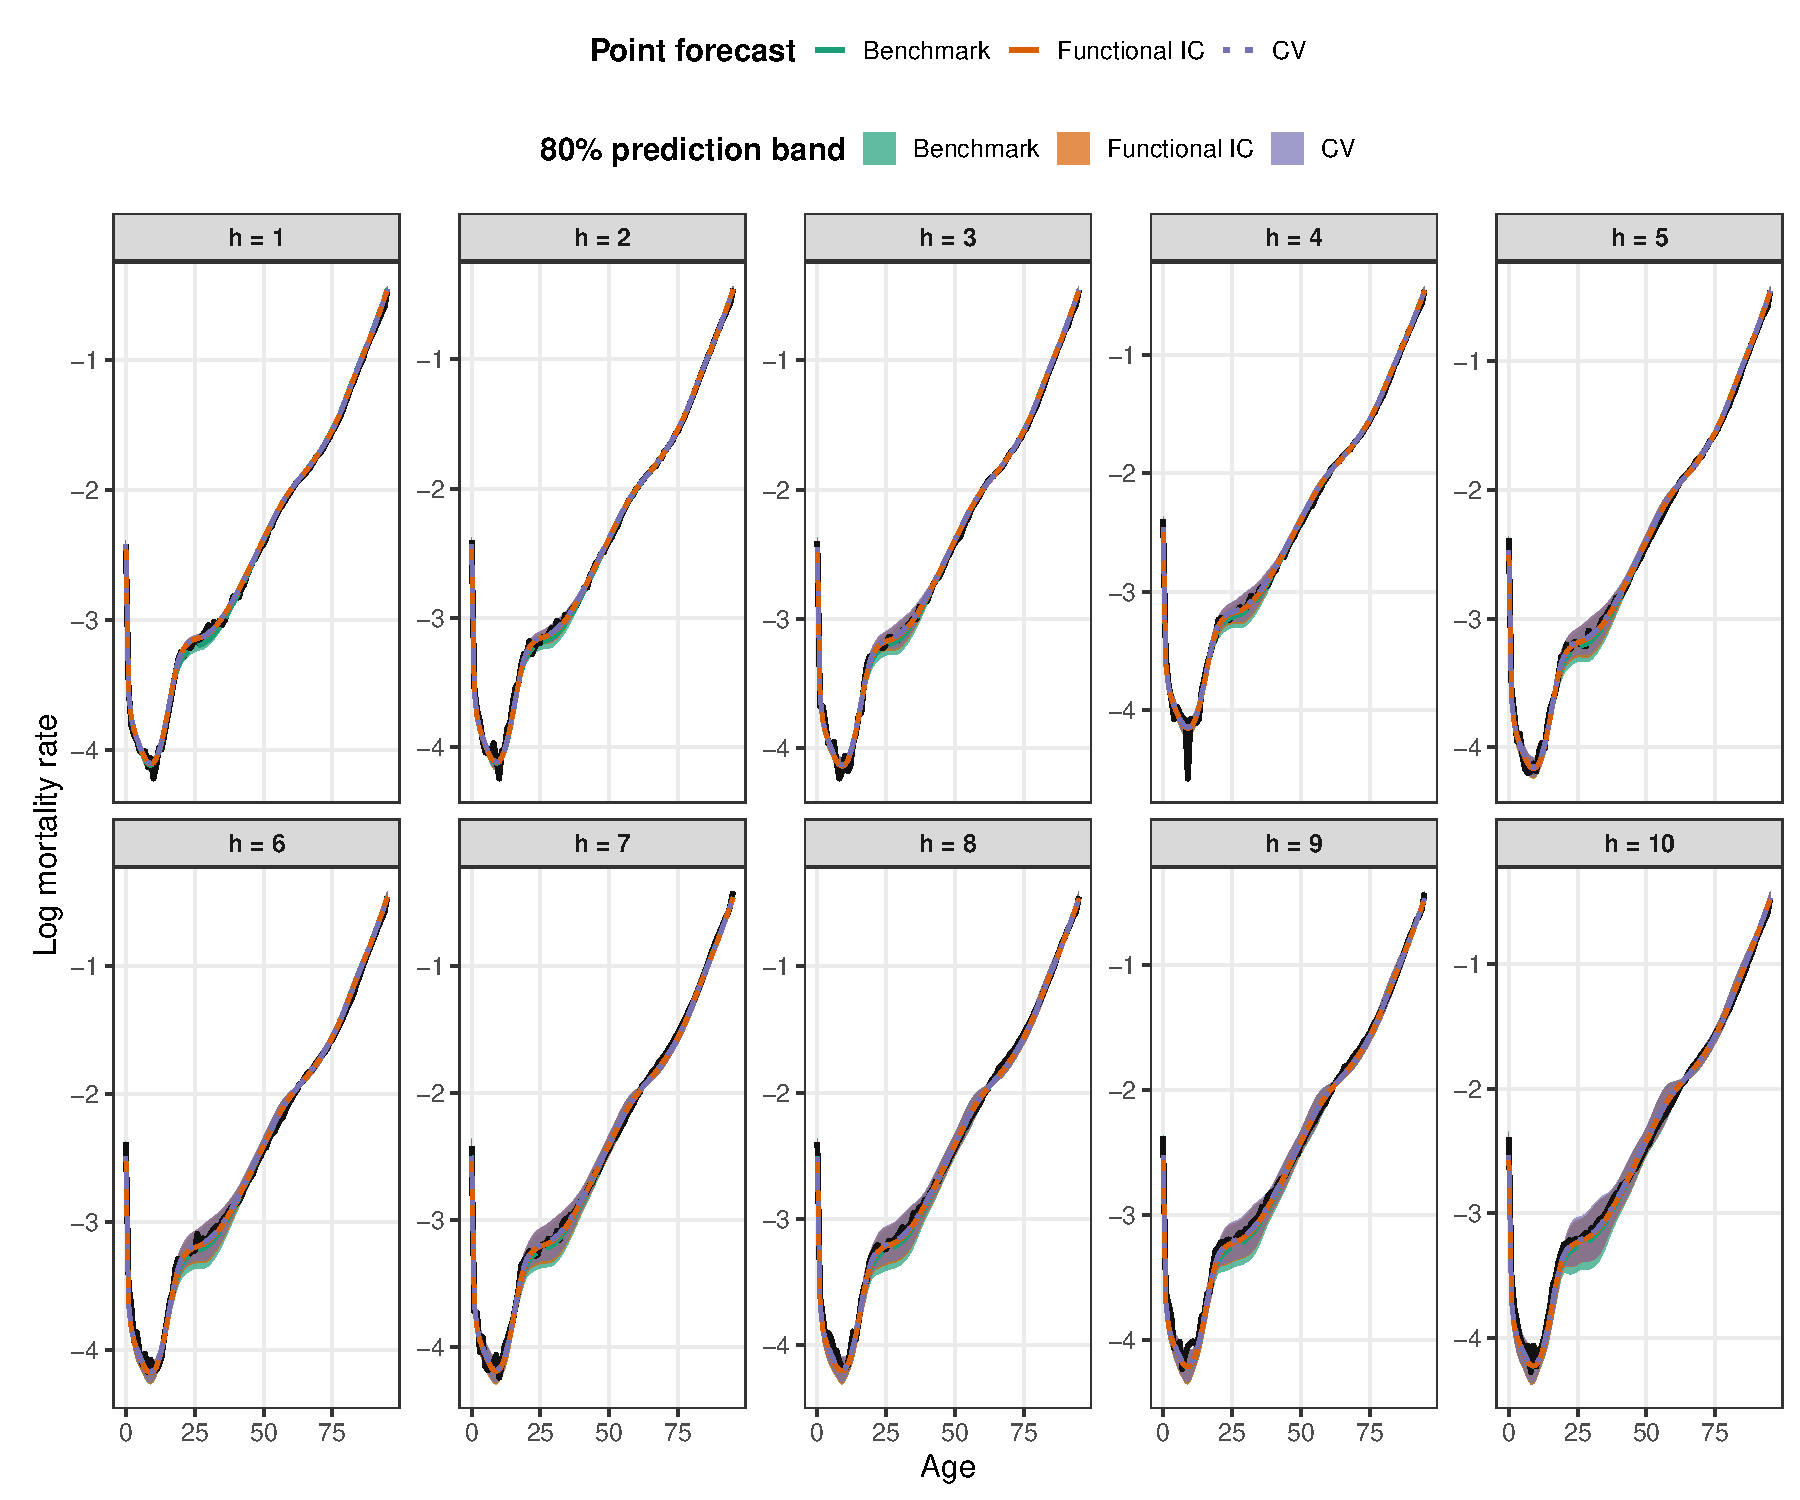
\includegraphics[width=0.98\textwidth]{Figures/Empirical/France_male_mortality_forecasts_80.pdf}
\caption{\small French male log-mortality forecasts for horizons $h=1,\ldots,10$ at the latest common test origin. Black solid lines are raw observed curves. Coloured lines are point forecasts, and each central 80\% prediction band uses the colour of its corresponding method.}
\label{fig:emp-male-mortality-forecast}
\end{figure}

\clearpage
\section{Comparison and Discussion}
\label{sec:emp-discussion}

The two empirical studies illustrate complementary benefits of the proposed framework. For fertility-rate changes, $\widehat d=0.3886$ is far from the benchmark value $d=1$, while the Functional IC and CV short-memory orders are similar. The large and nearly identical forecast gains from the two data-driven methods therefore point mainly to correct estimation of fractional integration. For mortality, $\widehat d$ is already close to one, so the smaller differences in performance arise mainly from selecting $(p,q)$. Functional IC improves both female and male forecasts without adopting the unnecessarily rich male order selected by CV.

This decomposition should be understood as an evidence-based interpretation rather than a formal causal attribution. A direct robustness check could compare models that vary only $d$ while fixing $(p,q)$ and models that vary only $(p,q)$ while fixing $d$. Even without that additional experiment, the contrast is informative: estimating $d$ matters most when the unit-integration benchmark is incompatible with the data, whereas adaptive selection of $(p,q)$ matters more when $d$ is already near one.

Two further qualifications are important. First, the fACF and fractional estimate provide evidence of persistence but are not a stand-alone test of the complete FARFIMA specification. Second, the intervals are calibrated from smoothed curves but assessed against raw observations. This is appropriate for evaluating observed demographic rates, but introduces measurement variation absent from the calibration target and is most visible in short-horizon mortality coverage. A useful sensitivity analysis would recalibrate nonconformity scores to raw validation curves or explicitly include an observation-error component.
